\subsection{Circuit Training}
\label{appendix:circuit_training}

This section shows the full set of metrics for the toy macro standard cell and Ariane netlists in the circuit training domain. The results highlight the differences in data cost, reliability, system performance, and application performance between behavioral cloning (BC), DDQN, and PPO.

\begin{table}[!htbp]
\centering
\resizebox{0.9\textwidth}{!}{%
\begin{tabular}{|l|l|c|c|c|}
\toprule
\multicolumn{5}{|c|}{\textbf{Toy Macro Standard Cell (Training)}} \\

 &  & \textbf{BC} & \textbf{DDQN} & \textbf{PPO} \\
\textbf{Category} & \textbf{Metric Name} &  &  &  \\
\midrule
\multirow[t]{1}{*}{Data Cost} & Training Sample Cost (kWh) & 4.44 & 0 & 0 \\
\midrule
\multirow[t]{2}{*}{Application} & Generalization (100 eps. [all tasks]) & -2.19 & -2.20 & -2.13 \\
 & Returns (100 eps.) & -0.97 $\pm$ \num{2.27e-03} & -1.05 $\pm$ 0.04 & -0.97 $\pm$ \num{8.09e-03} \\
\cline{1-5}
\multirow[t]{5}{*}{Reliability} & Dispersion Across Runs (IQR) & N/A & 0.01 $\pm$ 0.01 & 9.07e-03 $\pm$ \num{6.43e-03} \\
 & Dispersion Within Runs (IQR) & N/A & \num{8.80e-03} $\pm$ 0.01 & \num{2.51e-03} $\pm$ \num{3.61e-03} \\
 & Long Term Risk (CVaR) & N/A & 1.10 & 0.04 \\
 & Risk Across Runs (CVaR) & N/A & -1.08 & -0.99 \\
 & Short Term Risk (CVaR) & N/A & 0.03 & \num{9.89e-03} \\
\cline{1-5}
\multirow[t]{4}{*}{System} & Energy Consumed (kWh) & 0.02 $\pm$ \num{1.97e-04} & 5.55 $\pm$ 2.03 & 15.37 $\pm$ 3.79 \\
 & GPU Power Usage (W) & 188.20 $\pm$ 21.98 & 448.00 $\pm$ 200.41 & 307.05 $\pm$ 69.75 \\
 & Peak RAM Usage (GB) & 4.71 $\pm$ 0.02 & 525.99 $\pm$ 205.64 & 675.26 $\pm$ 45.30 \\
 & Wall Clock Time (Hours) & 0.10 $\pm$ \num{1.36e-03} & 0.29 $\pm$ 0.57 & 1.79 $\pm$ 2.16 \\
\cline{1-5}
\midrule
\multicolumn{5}{|c|}{\textbf{Toy Macro Standard Cell (Inference)}} \\
\multirow[t]{2}{*}{Reliability} & Dispersion Across Rollouts (IQR) & \num{1.68e-03} & 0.09 & \num{2.43e-03} \\
 & Risk Across Rollouts (CVaR) & -0.97 & -1.10 & -0.99 \\
\cline{1-5}
\multirow[t]{4}{*}{System} & GPU Power Usage (W) & 104.97 $\pm$ 22.85 & 59.45 $\pm$ 1.43 & 58.97 $\pm$ 1.14 \\
 % & Inference Time (ms) & 8.93e-03 $\pm$ 5.12e-04 & 0.02 $\pm$ 2.69e-03 & 0.02 $\pm$ 2.67e-03 \\
 & Inference Time (ms) & 8.93 $\pm$ 0.51 & 20 $\pm$ 2.69 & 20 $\pm$ 2.67 \\
 & Mean RAM Usage (GB) & 1.92 $\pm$ 0.42 & 1.45 $\pm$ 0.48 & 1.99 $\pm$ 0.30 \\
 & Peak RAM Usage (GB) & 2.14 $\pm$ 0.03 & 2.10 $\pm$ 0.05 & 2.16 $\pm$ 0.07 \\
\bottomrule
\end{tabular}
}

\caption{Metrics for the "Toy Macro" netlist task of CircuitTraining-v0. All metrics are averaged over ten random seeds. Note that the training reliability metrics for BC are marked as ``N/A'' since BC does not perform online rollouts in the environment.}
\label{tab:appendix_metrics_circuit_training_toy_macro_stdcell}
\end{table}


\begin{table}[H]
\resizebox{0.9\textwidth}{!}{%
\begin{tabular}{|l|l|c|c|c|}

\toprule
\multicolumn{5}{|c|}{\textbf{Ariane (Training)}} \\
 &  & \textbf{BC} & \textbf{DDQN} & \textbf{PPO} \\
\textbf{Category} & \textbf{Metric Name} &  &  &  \\
\midrule
\multirow[t]{1}{*}{Data Cost} & Training Sample Cost & 48.28 & 0 & 0 \\
\midrule
\multirow[t]{2}{*}{Application} & Generalization (100 eps. [all tasks]) & -2.18 & -2.19 & -2.05 \\
 & Returns (100 eps.) & -1.10 $\pm$ 0.04 & -1.13 $\pm$ 0.04 & -0.99 $\pm$ \num{7.25e-03} \\
\cline{1-5}
\multirow[t]{5}{*}{Reliability} & Dispersion Across Runs (IQR) & N/A & 0.03 $\pm$ 0.03 & 0.04 $\pm$ 0.02 \\
 & Dispersion Within Runs (IQR) & N/A & 0.02 $\pm$ 0.03 & \num{4.77e-03} $\pm$ \num{4.92e-03} \\
 & Long Term Risk (CVaR) & N/A & 1.20 & 0.03 \\
 & Risk Across Runs (CVaR) & N/A & -1.17 & -1.03 \\
 & Short Term Risk (CVaR) & N/A & 0.07 & 0.01 \\
\cline{1-5}
\multirow[t]{5}{*}{System} & Energy Consumed (kWh) & 0.11 $\pm$ \num{6.45e-04} & 108.20 $\pm$ 4.29 & 120.53 $\pm$ 2.78 \\

 & GPU Power Usage (W) & 211.35 $\pm$ 16.76 & 585.98 $\pm$ 172.50 & 692.94 $\pm$ 120.08 \\
 & Mean RAM Usage (GB) & 4.72 $\pm$ 0.53 & 849.37 $\pm$ 64.85 & 834.05 $\pm$ 55.90 \\
 & Peak RAM Usage (GB) & 5.25 $\pm$ 0.07 & 889.56 $\pm$ 23.44 & 906.45 $\pm$ 68.01 \\
 & Wall Clock Time (Hours) & 0.48 $\pm$ 2.61e-03 & 21.94 $\pm$ 0.90 & 23.95 $\pm$ 0.54 \\
\cline{1-5}
\midrule
\multicolumn{5}{|c|}{\textbf{Ariane (Inference)}} \\
\multirow[t]{2}{*}{Reliability} & Dispersion Across Rollouts (IQR) & 0.01 & 0.05 & 0.01 \\
 & Risk Across Rollouts (CVaR) & -1.23 & -1.25 & -1.01 \\
\cline{1-5}
\multirow[t]{4}{*}{System} & GPU Power Usage (W) & 136.91 $\pm$ 21.48 & 69.50 $\pm$ 4.60 & 49.43 $\pm$ 30.29 \\
 % & Inference Time (ms) & 0.01 $\pm$ 4.62e-04 & 0.02 $\pm$ 2.69e-03 & 0.02 $\pm$ 2.68e-03 \\
 & Inference Time (ms) & 10.0 $\pm$ 0.46 & 20.0 $\pm$ 2.69 & 20.0 $\pm$ 2.68 \\
 & Mean RAM Usage (GB) & 2.19 $\pm$ 0.21 & 2.15 $\pm$ 0.30 & 2.51 $\pm$ 0.49 \\
 & Peak RAM Usage (GB) & 2.29 $\pm$ 0.01 & 2.28 $\pm$ 0.13 & 2.71 $\pm$ 0.62 \\
\cline{1-5}
\bottomrule
\end{tabular}
}
% \vspace{0.5em}
\caption{Metrics for the Ariane Netlist task of CircuitTraining-v0. All metrics are averaged over ten random seeds. Note that the training reliability metrics for BC are marked as ``N/A'' since BC does not perform online rollouts in the environment.}
\label{tab:appendix_metrics_circuit_training_ariane}
\end{table}




\subsection{Quadruped Locomotion}
\label{appendix:quadruped_locomotion}

This section reports the metrics for the dog pace, trot, and spin gaits in the quadruped locomotion domain. The reliability metrics provide insights into the stability and worst-case performance of the algorithms during training and inference.

\begin{table}[H]
\resizebox{0.9\textwidth}{!}{%
\begin{tabular}{|l|l|c|c|c|}
\toprule
\multicolumn{5}{|c|}{\textbf{Dog Pace (Training)}} \\
 &  & \textbf{BC} & \textbf{PPO} & \textbf{SAC} \\
\textbf{Category} & \textbf{Metric Name} &  &  &  \\
\midrule
\multirow[t]{1}{*}{Data Cost} & Training Sample Cost (kWh) & 22.53 & 0 & 0 \\
\midrule
\multirow[t]{2}{*}{Application} & Generalization (100 eps. [all tasks]) & 3.99 & 3.36 & 5.03 \\
 & Returns (100 eps.) & 7.00 $\pm$ 4.68 & 9.94 $\pm$ 15.59 & 6.96 $\pm$ 6.72 \\
\cline{1-5}
\multirow[t]{5}{*}{Reliability} & Dispersion Across Runs (IQR) & N/A & 9.63 $\pm$ 7.27 & 3.61 $\pm$ 3.88 \\
 & Dispersion Within Runs (IQR) & N/A & 2.22 $\pm$ 1.97 & 2.98 $\pm$ 3.64 \\
 & Long Term Risk (CVaR) & N/A & 13.00 & 25.82 \\
 & Risk Across Runs (CVaR) & N/A & 13.74 & 8.55 \\
 & Short Term Risk (CVaR) & N/A & 5.81 & 10.19 \\
\cline{1-5}
\multirow[t]{5}{*}{System} & Energy Consumed (kWh) & 0.11 $\pm$ 0.02 & 32.46 $\pm$ 0.26 & 36.22 $\pm$ 2.33 \\
 & GPU Power Usage (W) & 240.64 $\pm$ 5.41 & 280.12 $\pm$ 23.69 & 266.37 $\pm$ 9.54 \\
 & Mean RAM Usage (GB) & 3.21 $\pm$ 0.24 & 532.93 $\pm$ 14.28 & 516.24 $\pm$ 75.03 \\
 & Peak RAM Usage (GB) & 3.25 $\pm$ 0.01 & 534.26 $\pm$ 2.04 & 545.16 $\pm$ 0.50 \\
 & Wall Clock Time (Hours) & 0.46 $\pm$ 0.07 & 18.73 $\pm$ 0.19 & 19.41 $\pm$ 2.74 \\
\cline{1-5}
\midrule
\multicolumn{5}{|c|}{\textbf{Dog Pace (Inference)}} \\
\multirow[t]{2}{*}{Reliability} & Dispersion Across Rollouts (IQR) & 0.52 & 8.76 & 4.80 \\
 & Risk Across Rollouts (CVaR) & 0.33 & 0.46 & 1.69 \\
\cline{1-5}
\multirow[t]{4}{*}{System} & GPU Power Usage (W) & 60.37 $\pm$ 1.78 & 59.11 $\pm$ 1.31 & 61.41 $\pm$ 1.96 \\
 % & Inference Time (ms) & 2.33e-03 $\pm$ 5.38e-04 & 2.56e-03 $\pm$ 3.92e-04 & 2.52e-03 $\pm$ 7.35e-04 \\
 & Inference Time (ms) & 2.33 $\pm$ 0.54 & 2.56 $\pm$ 0.39 & 2.52 $\pm$ 0.74 \\

 & Mean RAM Usage (GB) & 1.69 $\pm$ 0.31 & 1.81 $\pm$ 0.14 & 1.71 $\pm$ 0.30 \\
 & Peak RAM Usage (GB) & 1.82 $\pm$ 0.03 & 1.84 $\pm$ 9.05e-03 & 1.85 $\pm$ 0.04 \\
\bottomrule
\end{tabular}
}
% \vspace{0.5em}
\caption{Metrics for the "dog pace" gait of QuadrupedLocomotion-v0. All metrics are averaged over ten random seeds. Note that the training reliability metrics for BC are marked as ``N/A'' since BC does not perform online rollouts in the environment.}
\label{tab:appendix_locomotion_dog_pace}
\end{table}


\begin{table}[!htbp]
\resizebox{0.95\linewidth}{!}{%
\begin{tabular}{|l|l|c|c|c|}
\toprule
\multicolumn{5}{|c|}{\textbf{Dog Trot (Training)}} \\
 &  & \textbf{BC} & \textbf{PPO} & \textbf{SAC} \\
\textbf{Category} & \textbf{Metric Name} &  &  &  \\
\midrule
\multirow[t]{1}{*}{Data Cost} & Training Sample Cost (kWh) & 15.77 & 0 & 0 \\
\midrule
\multirow[t]{2}{*}{Application} & Generalization (100 eps. [all tasks]) & 3.87 & 3.09 & 4.49 \\
 & Returns (100 eps.) & 1.06 $\pm$ 0.26 & 1.49 $\pm$ 1.02 & 3.51 $\pm$ 2.88 \\
\cline{1-5}
\multirow[t]{5}{*}{Reliability} & Dispersion Across Runs (IQR) & N/A & 9.07 $\pm$ 4.93 & 0.85 $\pm$ 1.29 \\
 & Dispersion Within Runs (IQR) & N/A & 0.82 $\pm$ 0.84 & 0.93 $\pm$ 1.11 \\
 & Long Term Risk (CVaR) & N/A & 6.79 & 8.46 \\
 & Risk Across Runs (CVaR) & N/A & 6.00 & 2.58 \\
 & Short Term Risk (CVaR) & N/A & 2.41 & 3.20 \\
\cline{1-5}
\multirow[t]{5}{*}{System} & Energy Consumed (kWh) & 0.12 $\pm$ 0.02 & 16.82 $\pm$ 0.29 & 19.17 $\pm$ 0.64 \\
 & GPU Power Usage (W) & 242.12 $\pm$ 7.53 & 277.71 $\pm$ 23.47 & 269.18 $\pm$ 10.12 \\
 & Mean RAM Usage (GB) & 3.21 $\pm$ 0.25 & 535.00 $\pm$ 18.77 & 535.99 $\pm$ 29.49 \\
 & Peak RAM Usage (GB) & 3.26 $\pm$ 0.01 & 536.47 $\pm$ 1.98 & 544.80 $\pm$ 4.39 \\
 & Wall Clock Time (Hours) & 0.46 $\pm$ 0.06 & 18.57 $\pm$ 0.23 & 18.99 $\pm$ 6.78 \\
\cline{1-5}
\midrule
\multicolumn{5}{|c|}{\textbf{Dog Trot (Inference)}} \\
\multirow[t]{2}{*}{Reliability} & Dispersion Across Rollouts (IQR) & 0.32 & 0.89 & 1.25 \\
 & Risk Across Rollouts (CVaR) & 0.63 & 0.36 & 1.33 \\
\cline{1-5}
\multirow[t]{4}{*}{System} & GPU Power Usage (W) & 59.32 $\pm$ 1.08 & 58.91 $\pm$ 1.28 & 59.39 $\pm$ 1.23 \\
 % & Inference Time (ms) & 2.32e-03 $\pm$ 4.94e-04 & 2.55e-03 $\pm$ 5.74e-04 & 2.45e-03 $\pm$ 3.54e-04 \\

 & Inference Time (ms) & 2.32 $\pm$ 0.49 & 2.55 $\pm$ 0.57 & 2.45 $\pm$ 0.35 \\

 & Mean RAM Usage (GB) & 1.66 $\pm$ 0.33 & 1.76 $\pm$ 0.25 & 1.80 $\pm$ 0.17 \\
 & Peak RAM Usage (GB) & 1.82 $\pm$ \num{8.77e-04} & 1.85 $\pm$ 0.02 & 1.85 $\pm$ 0.03 \\
\bottomrule
\end{tabular}
}
% \vspace{0.5em}
\caption{Metrics for the "dog trot" gait of QuadrupedLocomotion-v0. All metrics are averaged over ten random seeds. Note that the training reliability metrics for BC are marked as ``N/A'' since BC does not perform online rollouts in the environment.}
\label{tab:appendix_locomotion_dog_trot}
\end{table}


\begin{table}[!htbp]
\resizebox{0.95\linewidth}{!}{%
\begin{tabular}{|l|l|c|c|c|}
\toprule
\multicolumn{5}{|c|}{\textbf{Dog Spin (Training)}} \\
 &  & \textbf{BC} & \textbf{PPO} & \textbf{SAC} \\
\textbf{Category} & \textbf{Metric Name} &  &  &  \\
\midrule
\multirow[t]{1}{*}{Data Cost} & Training Sample Cost (kWh) &30.17 & 0 & 0 \\
\midrule
\multirow[t]{2}{*}{Application} & Generalization (100 eps. [all tasks]) & 3.97 & 2.69 & 4.61 \\
 & Returns (100 eps.) & 1.54 $\pm$ 0.42 & 3.82 $\pm$ 6.22 & 3.84 $\pm$ 1.46 \\
\cline{1-5}
\multirow[t]{5}{*}{Reliability} & Dispersion Across Runs (IQR) & N/A & 7.92 $\pm$ 4.60 & 0.74 $\pm$ 0.76 \\
 & Dispersion Within Runs (IQR) & N/A & 1.00 $\pm$ 1.08 & 0.84 $\pm$ 1.26 \\
 & Long Term Risk (CVaR) & N/A & 8.88 & 14.37 \\
 & Risk Across Runs (CVaR) & N/A & 8.29 & 3.82 \\
 & Short Term Risk (CVaR) & N/A & 3.09 & 2.99 \\
\cline{1-5}
\multirow[t]{5}{*}{System} & Energy Consumed (kWh) & 0.10 $\pm$ 0.04 & 17.42 $\pm$ 0.35 & 18.88 $\pm$ 0.59 \\
 & GPU Power Usage (W) & 216.72 $\pm$ 68.63 & 278.38 $\pm$ 22.60 & 264.46 $\pm$ 9.49 \\
 & Mean RAM Usage (GB) & 3.18 $\pm$ 0.26 & 534.56 $\pm$ 21.28 & 531.27 $\pm$ 55.64 \\
 & Peak RAM Usage (GB) & 3.23 $\pm$ 0.08 & 536.10 $\pm$ 3.03 & 477.22 $\pm$ 172.63 \\
 & Wall Clock Time (Hours) & 0.45 $\pm$ 0.08 & 17.13 $\pm$ 6.07 & 17.02 $\pm$ 9.05 \\
\cline{1-5}
\midrule
\multicolumn{5}{|c|}{\textbf{Dog Spin (Inference)}} \\
\multirow[t]{2}{*}{Reliability} & Dispersion Across Rollouts (IQR) & 0.37 & 2.41 & 1.78 \\
 & Risk Across Rollouts (CVaR) & 0.28 & 0.12 & 0.55 \\
\cline{1-5}
\multirow[t]{4}{*}{System} & GPU Power Usage (W) & 60.10 $\pm$ 1.14 & 59.70 $\pm$ 1.22 & 59.65 $\pm$ 1.73 \\
 % & Inference Time (ms) & 2.33e-03 $\pm$ 6.63e-04 & 2.45e-03 $\pm$ 4.84e-04 & 2.41e-03 $\pm$ 2.24e-04 \\
 & Inference Time (ms) & 2.33 $\pm$ 0.66 & 2.45 $\pm$ 0.48 & 2.41 $\pm$ 0.22 \\

 & Mean RAM Usage (GB) & 1.68 $\pm$ 0.32 & 1.79 $\pm$ 0.22 & 1.75 $\pm$ 0.26 \\
 & Peak RAM Usage (GB) & 1.82 $\pm$ 0.03 & 1.85 $\pm$ 0.02 & 1.84 $\pm$ 0.02 \\
\bottomrule
\end{tabular}
}
% \vspace{0.5em}
\caption{Metrics for the "dog spin" gait of QuadrupedLocomotion-v0. All metrics are averaged over ten random seeds. Note that the training reliability metrics for BC are marked as ``N/A'' since BC does not perform online rollouts in the environment.}
\label{tab:appendix_locomotion_dog_spin}

\end{table}



\subsection{Web Navigation}
\label{appendix:web_navigation}

This section details the evaluation on websites of varying difficulty levels in the web navigation domain. The system performance metrics underscore the significant computational requirements, especially in terms of RAM usage, for training web navigation agents.

\begin{table}[!htbp]
\resizebox{0.95\linewidth}{!}{%
\begin{tabular}{|l|l|c|c|c|}
\toprule
\multicolumn{5}{|c|}{\textbf{Difficulty 1, 1 Website (Training)}} \\
 &  & \textbf{BC} & \textbf{DDQN} & \textbf{PPO} \\
\textbf{Category} & \textbf{Metric Name} &  &  &  \\
\midrule
\multirow[t]{1}{*}{Data Cost} & Training Sample Cost (kWh) & 14.15 & 0 & 0 \\
\midrule
\multirow[t]{2}{*}{Application} & Generalization (100 eps. [all tasks]) & -12.94 & -11.15 & -24.54 \\
 & Returns (100 eps.) & -3.57 $\pm$ 2.80 & -7.55 $\pm$ 5.74 & -13.45 $\pm$ 0.51 \\
\cline{1-5}
\multirow[t]{5}{*}{Reliability} & Dispersion Across Runs (IQR) & N/A & 0.73 $\pm$ 0.63 & 4.20 $\pm$ 1.45 \\
 & Dispersion Within Runs (IQR) & N/A & 0.37 $\pm$ 0.68 & 0.57 $\pm$ 0.53 \\
 & Long Term Risk (CVaR) & N/A & 9.32 & 12.12 \\
 & Risk Across Runs (CVaR) & N/A & -2.75 & -13.11 \\
 & Short Term Risk (CVaR) & N/A & 1.79 & 1.86 \\
\cline{1-5}
\multirow[t]{5}{*}{System} & Energy Consumed (kWh) & 0.04 $\pm$ \num{6.02e-04} & 29.56 $\pm$ 7.23 & 28.82 $\pm$ 1.19 \\
 & GPU Power Usage (W) & 125.89 $\pm$ 2.53 & 265.09 $\pm$ 21.50 & 305.15 $\pm$ 34.41 \\
 & Mean RAM Usage (GB) & 4.10 $\pm$ 0.33 & 1140.98 $\pm$ 580.55 & 1592.45 $\pm$ 388.64 \\
 & Peak RAM Usage (GB) & 4.23 $\pm$ 0.04 & 1931.54 $\pm$ 242.31 & 2305.57 $\pm$ 135.48 \\
 & Wall Clock Time (Hours) & 0.31 $\pm$ \num{4.91e-03} & 8.13 $\pm$ 5.17 & 10.50 $\pm$ 0.44 \\
\cline{1-5}
\midrule
\multicolumn{5}{|c|}{\textbf{Difficulty 1, 1 Website (Inference)}} \\
\multirow[t]{2}{*}{Reliability} & Dispersion Across Rollouts (IQR) & 3.36 & 11.75 & 0.50 \\
 & Risk Across Rollouts (CVaR) & -10.65 & -13.25 & -13.75 \\
\cline{1-5}
\multirow[t]{4}{*}{System} & GPU Power Usage (W) & 108.61 $\pm$ 15.76 & 59.61 $\pm$ 1.41 & 60.26 $\pm$ 1.14 \\
 % & Inference Time (ms) & 3.07e-03 $\pm$ 4.69e-04 & 0.11 $\pm$ 9.93e-03 & 0.12 $\pm$ 9.71e-03 \\
 & Inference Time (ms) & 3.07 $\pm$ 0.47 & 110 $\pm$ 9.93 & 120 $\pm$ 9.71 \\

 & Mean RAM Usage (GB) & 1.97 $\pm$ 0.32 & 2.08 $\pm$ 0.20 & 2.12 $\pm$ 0.17 \\
 & Peak RAM Usage (GB) & 2.11 $\pm$ 0.11 & 2.18 $\pm$ 0.11 & 2.19 $\pm$ 0.09 \\
\cline{1-5}
\bottomrule
\end{tabular}
}
% \vspace{0.5em}
\caption{Metrics for "difficulty 1, 1 website" task of WebNavigation-v0. All metrics are averaged over ten random seeds. Note that the training reliability metrics for BC are marked as ``N/A'' since BC does not perform online rollouts in the environment.}
\label{tab:appendix_metrics_webnav_difficulty_1_websites_1}
\end{table}


\begin{table}[!htbp]
\resizebox{0.95\linewidth}{!}{%
\begin{tabular}{|l|l|c|c|c|}
\toprule
\multicolumn{5}{|c|}{\textbf{Difficulty 1, 5 Websites (Training)}} \\
 &  & \textbf{BC} & \textbf{DDQN} & \textbf{PPO} \\
\textbf{Category} & \textbf{Metric Name} &  &  &  \\
\midrule
\multirow[t]{1}{*}{Data Cost} & Training Sample Cost (kWh) & 13.66 & 0 & 0 \\
\midrule
\multirow[t]{2}{*}{Application} & Generalization (100 eps. [all tasks]) & -13.34 & -11.03 & -23.86 \\
 & Returns (100 eps.) & -4.87 $\pm$ 3.33 & -3.43 $\pm$ 4.58 & -12.37 $\pm$ 3.53 \\
\cline{1-5}
\multirow[t]{5}{*}{Reliability} & Dispersion Across Runs (IQR) & N/A & 0.43 $\pm$ 0.55 & 3.42 $\pm$ 1.08 \\
 & Dispersion Within Runs (IQR) & N/A & 0.49 $\pm$ 0.97 & 0.75 $\pm$ 0.55 \\
 & Long Term Risk (CVaR) & N/A & 11.27 & 11.70 \\
 & Risk Across Runs (CVaR) & N/A & -1.26 & -12.60 \\
 & Short Term Risk (CVaR) & N/A & 2.47 & 2.05 \\
\cline{1-5}
\multirow[t]{5}{*}{System} & Energy Consumed (kWh) & 0.04 $\pm$ \num{4.82e-04} & 31.59 $\pm$ 5.19 & 28.48 $\pm$ 1.22 \\
 & GPU Power Usage (W) & 126.04 $\pm$ 4.03 & 265.81 $\pm$ 22.08 & 303.28 $\pm$ 34.99 \\
 & Mean RAM Usage (GB) & 4.03 $\pm$ 0.34 & 1206.86 $\pm$ 466.37 & 1545.56 $\pm$ 427.22 \\
 & Peak RAM Usage (GB) & 4.15 $\pm$ 0.11 & 1928.69 $\pm$ 209.62 & 2227.07 $\pm$ 210.77 \\
 & Wall Clock Time (Hours) & 0.30 $\pm$ \num{3.71e-03} & 9.35 $\pm$ 4.70 & 10.45 $\pm$ 0.31 \\

\cline{1-5}
\midrule
\multicolumn{5}{|c|}{\textbf{Difficulty 1, 5 Websites (Inference)}} \\

\multirow[t]{2}{*}{Reliability} & Dispersion Across Rollouts (IQR) & 5.96 & 0.29 & 0.50 \\
 & Risk Across Rollouts (CVaR) & -11.36 & -13.46 & -13.75 \\
\cline{1-5}
\multirow[t]{4}{*}{System} & GPU Power Usage (W) & 108.13 $\pm$ 16.85 & 60.87 $\pm$ 5.78 & 60.17 $\pm$ 1.67 \\
 % & Inference Time (ms) & 3.04e-03 $\pm$ 4.37e-04 & 0.11 $\pm$ 9.83e-03 & 0.12 $\pm$ 9.21e-03 \\
 & Inference Time (ms) & 3.04 $\pm$ 0.44 & 110 $\pm$ 9.83 & 120 $\pm$ 9.21 \\

 & Mean RAM Usage (GB) & 1.97 $\pm$ 0.33 & 2.07 $\pm$ 0.32 & 2.12 $\pm$ 0.16 \\
 & Peak RAM Usage (GB) & 2.12 $\pm$ 0.03 & 2.57 $\pm$ 0.86 & 2.19 $\pm$ 0.01 \\
\cline{1-5}
\bottomrule
\end{tabular}
}
% \vspace{0.5em}
\caption{Metrics for "difficulty 1, 5 websites" task of WebNavigation-v0. All metrics are averaged over ten random seeds. Note that the training reliability metrics for BC are marked as ``N/A'' since BC does not perform online rollouts in the environment.}
\label{tab:appendix_metrics_webnav_difficulty_1_websites_5}
\end{table}

% \usepackage{graphicx}

\begin{table}[H]
\centering
\resizebox{\textwidth}{!}{%
\begin{tabular}{|l|l|c|c|c|}
\toprule
\multicolumn{5}{|c|}{\textbf{Difficulty 1, 10 Websites (Training)}} \\
 &  & \textbf{BC} & \textbf{DDQN} & \textbf{PPO} \\
\textbf{Category} & \textbf{Metric Name} &  &  &  \\
\midrule
\multirow[t]{1}{*}{Data Cost} & Training Sample Cost (kWh) & 19.71 & 0 & 0 \\
\midrule
Application & Returns (100 eps.) & -4.68 $\pm$ 3.28 & -3.14 $\pm$ 4.24 & -12.73 $\pm$ 2.86 \\
\cline{1-5}
\multirow[t]{5}{*}{Reliability} & Dispersion Across Runs (IQR) & N/A & 0.32 $\pm$ 0.47 & 3.67 $\pm$ 0.63 \\
 & Dispersion Within Runs (IQR) & N/A & 0.42 $\pm$ 0.86 & 0.79 $\pm$ 0.53 \\
 & Long Term Risk (CVaR) & N/A & 9.47 & 11.85 \\
 & Risk Across Runs (CVaR) & N/A & -1.44 & -12.79 \\
 & Short Term Risk (CVaR) & N/A & 2.27 & 1.82 \\
\cline{1-5}
\multirow[t]{5}{*}{System} & Energy Consumed (kWh) & 0.05 $\pm$ \num{2.41e-04} & 27.19 $\pm$ 11.22 & 20.35 $\pm$ 5.77 \\
 & GPU Power Usage (W) & 125.88 $\pm$ 2.33 & 264.98 $\pm$ 24.45 & 304.66 $\pm$ 33.77 \\
 & Mean RAM Usage (GB) & 3.56 $\pm$ 0.39 & 1214.88 $\pm$ 524.77 & 1034.85 $\pm$ 424.83 \\
 & Peak RAM Usage (GB) & 4.10 $\pm$ 0.05 & 1784.37 $\pm$ 641.82 & 1665.15 $\pm$ 395.14 \\
 & Wall Clock Time (Hours) & 0.32 $\pm$ 1.43e-03 & 7.80 $\pm$ 5.20 & 3.10 $\pm$ 5.06 \\
\cline{1-5}
\midrule
\multicolumn{5}{|c|}{\textbf{Difficulty 1, 10 Websites (Inference)}} \\
\multirow[t]{2}{*}{Reliability} & Dispersion Across Rollouts (IQR) & 5.86 & 0.25 & 0.50 \\
 & Risk Across Rollouts (CVaR) & -11.33 & -13.28 & -13.75 \\
\cline{1-5}
\multirow[t]{4}{*}{System} & GPU Power Usage (W) & 108.26 $\pm$ 16.34 & 59.95 $\pm$ 1.49 & 59.67 $\pm$ 1.57 \\
 % & Inference Time (ms) & 3.05e-03 $\pm$ 4.46e-04 & 0.11 $\pm$ 8.42e-03 & 0.12 $\pm$ 9.90e-03 \\
 & Inference Time (ms) & 3.05 $\pm$ 0.45 & 110 $\pm$ 8.42 & 120 $\pm$ 9.90 \\

 & Mean RAM Usage (GB) & 1.97 $\pm$ 0.35 & 2.06 $\pm$ 0.27 & 2.13 $\pm$ 0.16 \\
 & Peak RAM Usage (GB) & 2.13 $\pm$ 0.04 & 2.17 $\pm$ 0.03 & 2.20 $\pm$ 0.03 \\
\cline{1-5}
\bottomrule
\end{tabular}
} % End of \resizebox
% \vspace{0.5em}
\caption{Metrics for "difficulty 1, 10 websites" task of WebNavigation-v0. All metrics are averaged over ten random seeds. Note that the training reliability metrics for BC are marked as ``N/A'' since BC does not perform online rollouts in the environment.}
\label{tab:appendix_metrics_webnav_difficulty_1_websites_10}
\end{table}

\pagebreak
\subsection{Radar Plots for Easy Visual Comparison}
\label{appendix:radar_plots}

These figures provide a graphical representation of the key metrics across all domains and tasks, enabling a visual comparison of the algorithms' performance along the different evaluation axes.


% % ---- Locomotion Spin
% \begin{figure}[H]
%   \centering
%   \begin{minipage}[b]{0.53\linewidth}
%     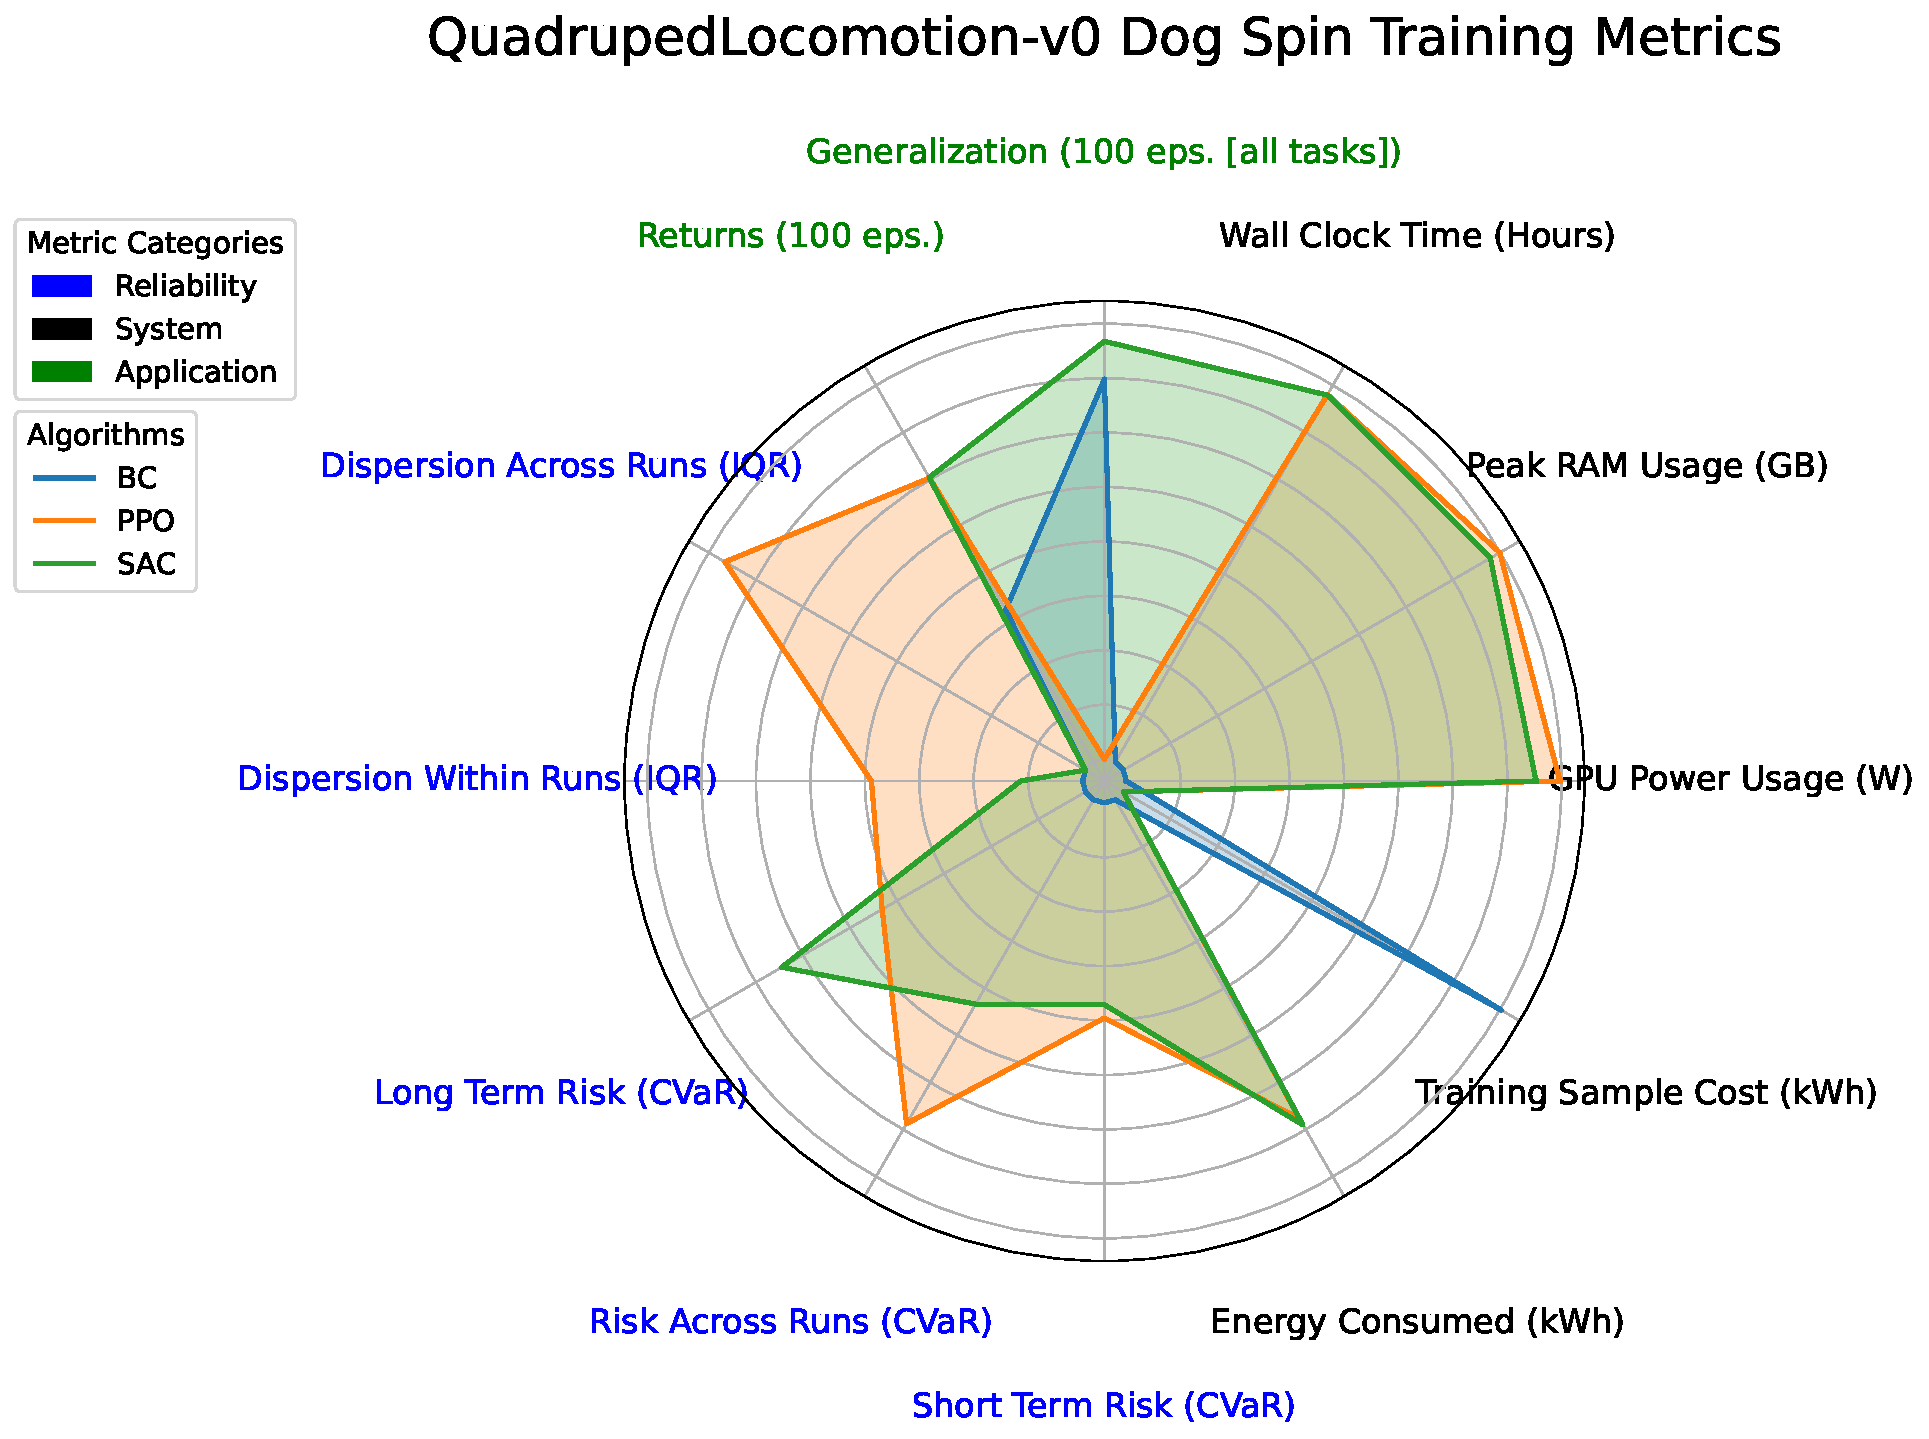
\includegraphics[width=\linewidth]{img/quadruped_locomotion/QuadrupedLocomotion-v0 Dog Spin Training Metrics.pdf}
%     \caption{Locomotion Spin Training Metrics}
%     \label{fig:image1}
%   \end{minipage}
%   \hfill % optional; adds horizontal spacing
%   \begin{minipage}[b]{0.4625\linewidth}
%     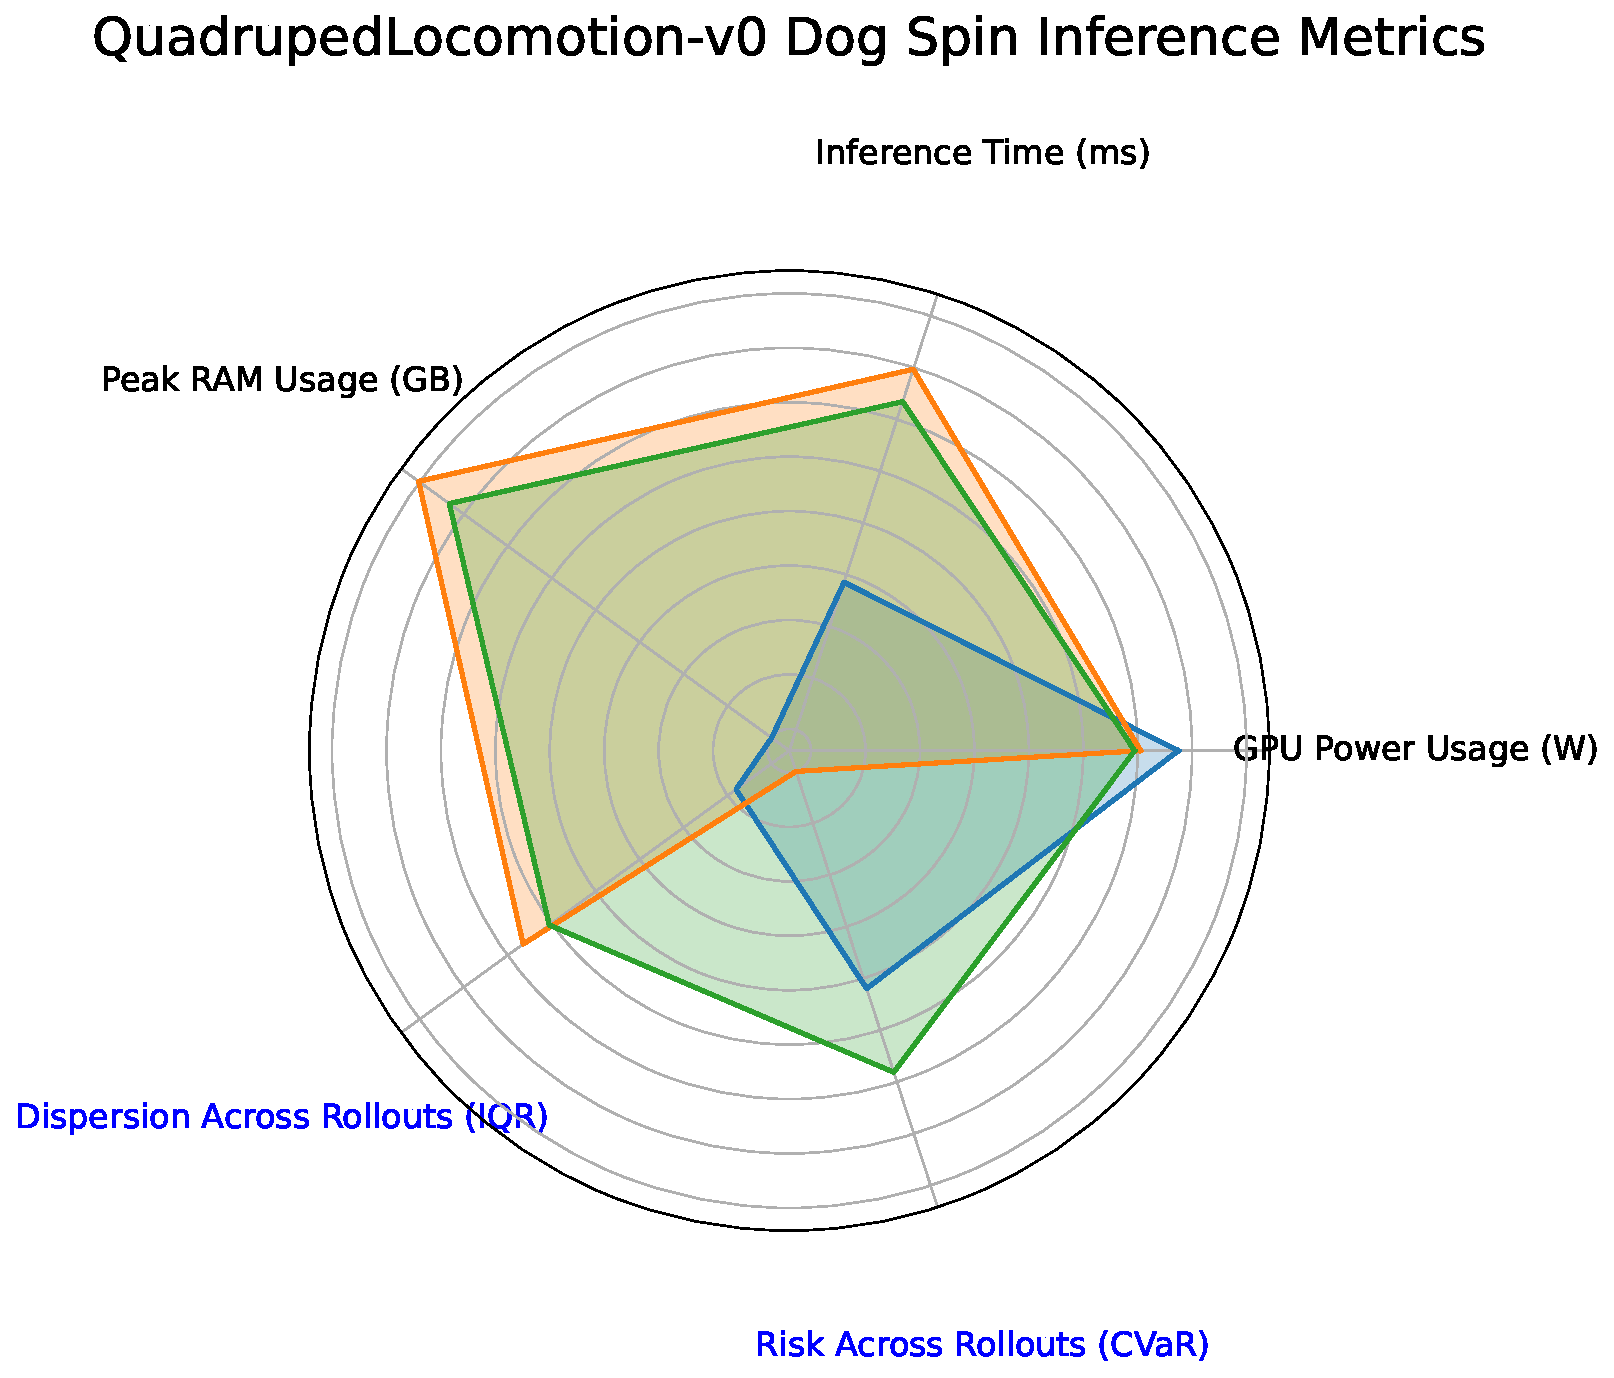
\includegraphics[width=\linewidth]{img/quadruped_locomotion/QuadrupedLocomotion-v0 Dog Spin Inference Metrics.pdf}
%     \caption{Locomotion Spin Inference Metrics}
%     \label{fig:image2}
%   \end{minipage}
% \end{figure}
% ---- Locomotion Spin
\begin{figure}[!htbp]
  \centering
  \begin{minipage}[b]{0.53\linewidth}
    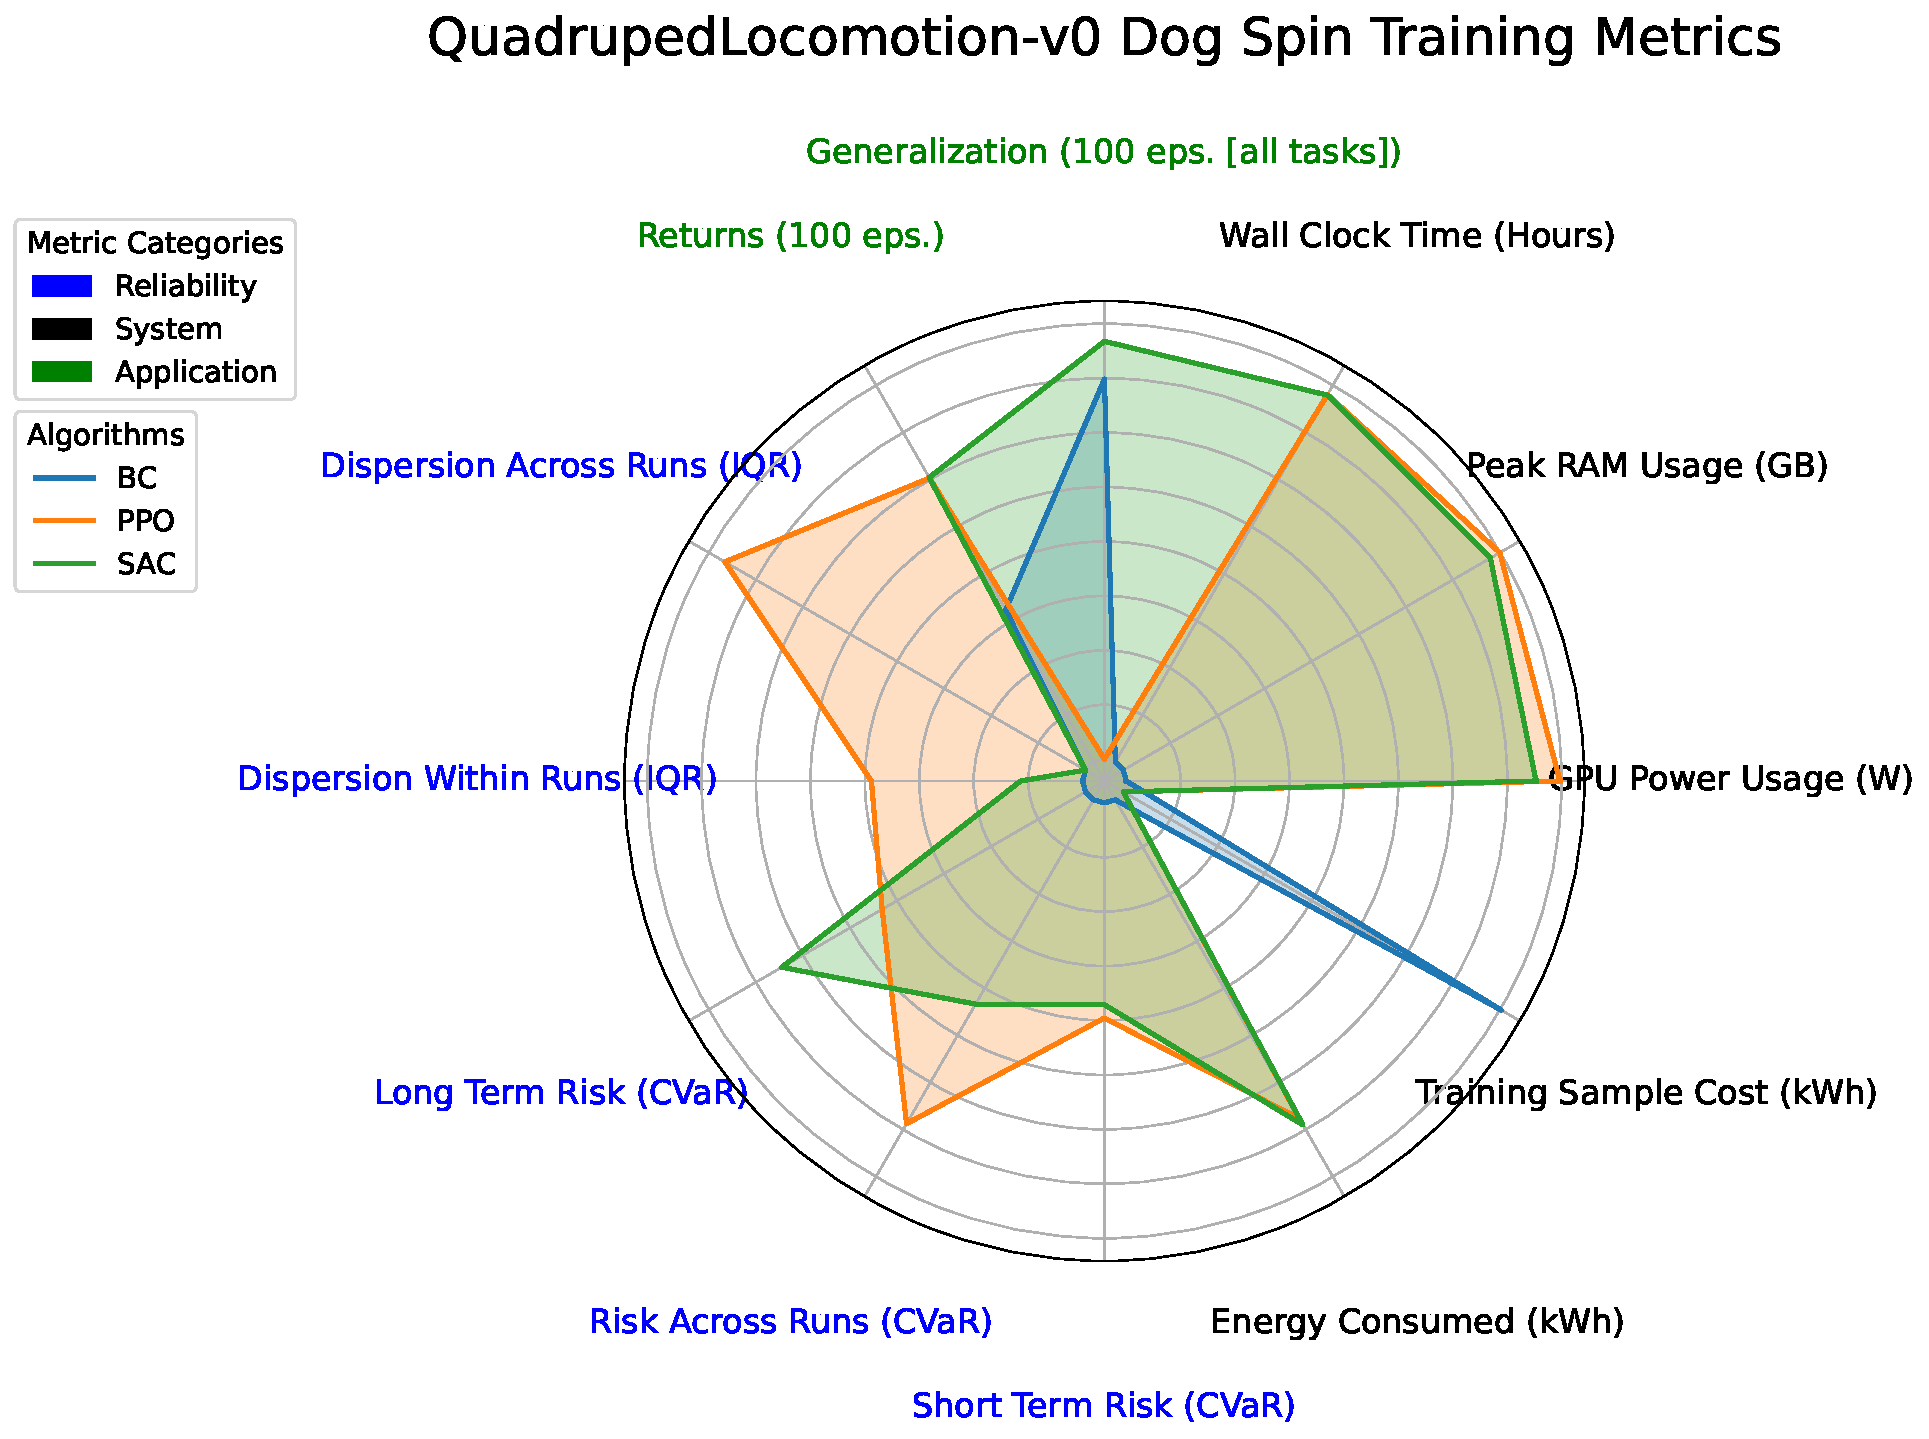
\includegraphics[width=\linewidth]{img/quadruped_locomotion/QuadrupedLocomotion-v0 Dog Spin Training Metrics.pdf}
  \end{minipage}
  \hfill % optional; adds horizontal spacing
  \begin{minipage}[b]{0.4625\linewidth}
    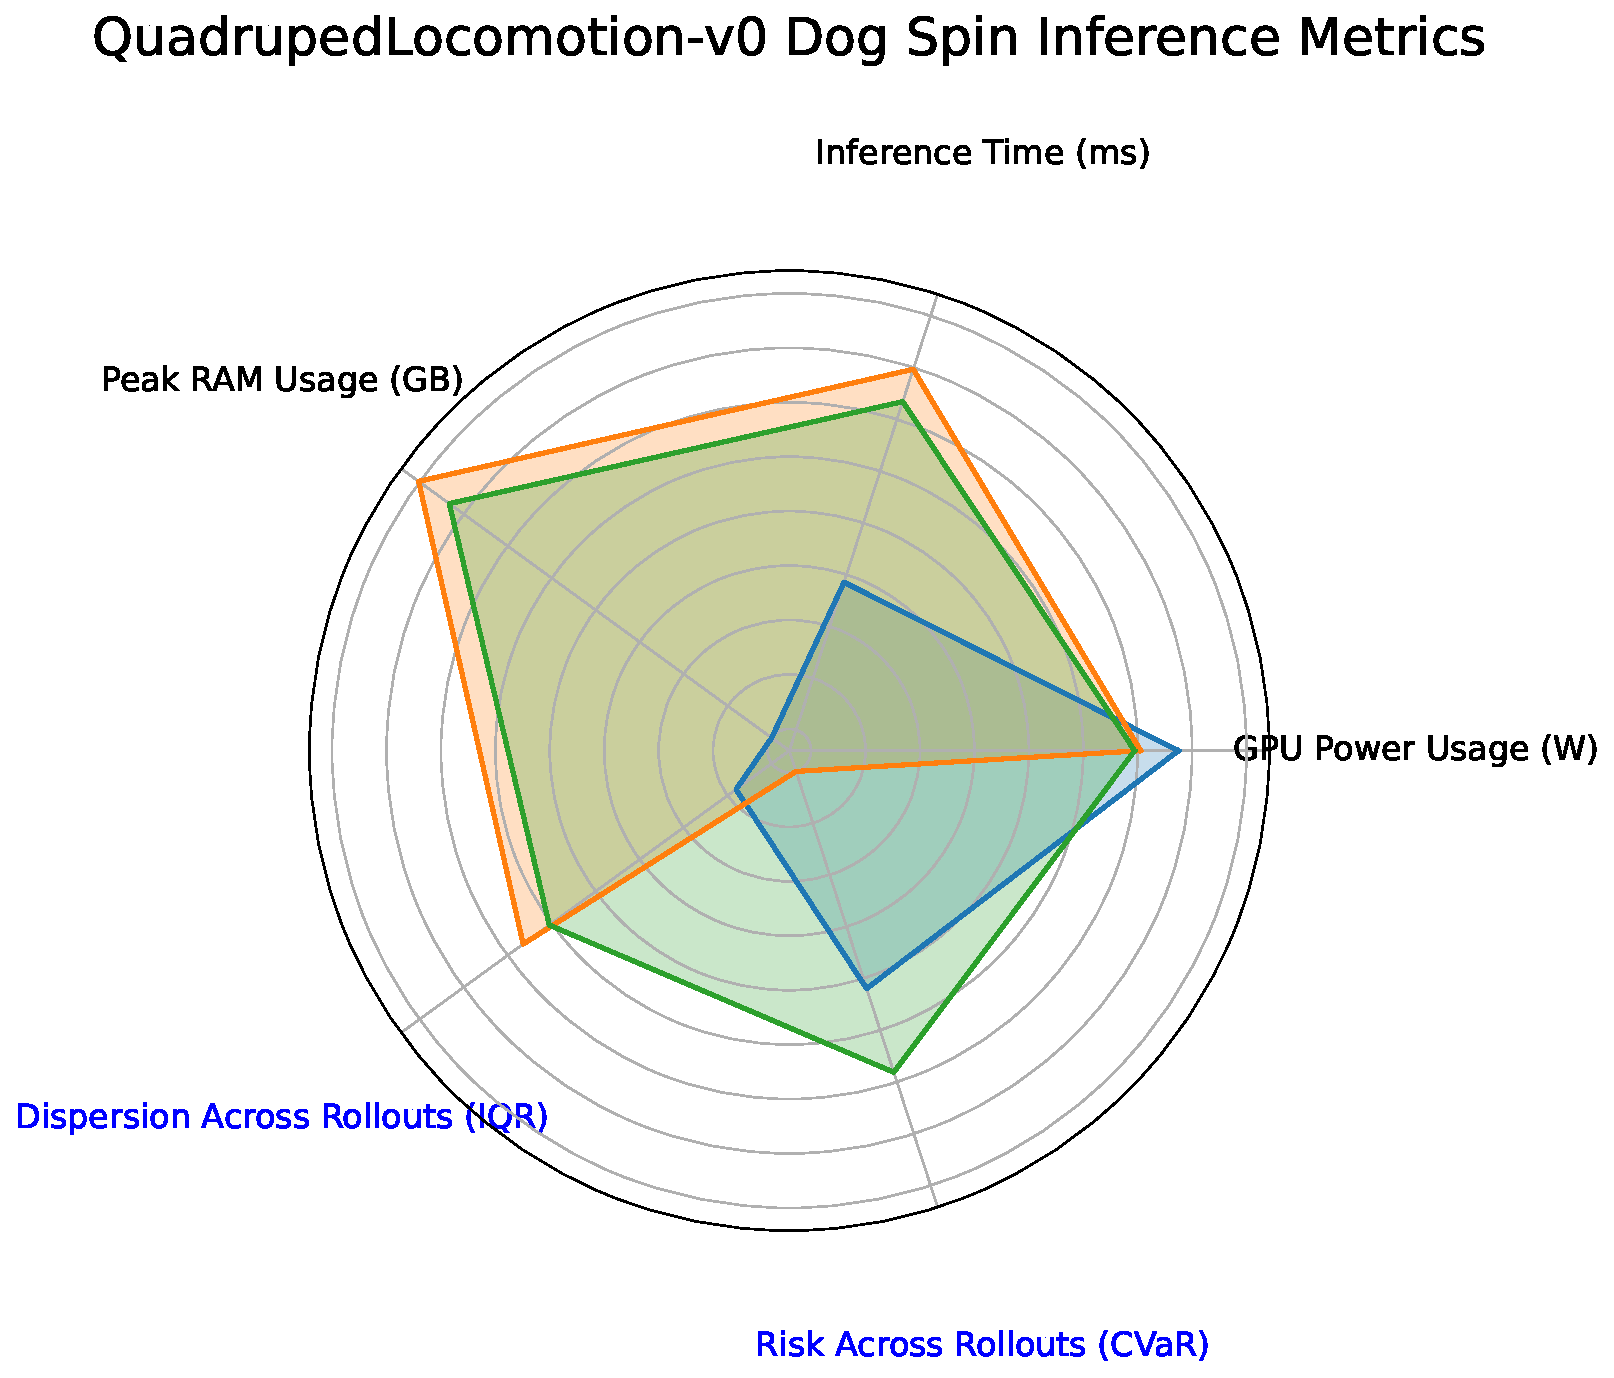
\includegraphics[width=\linewidth]{img/quadruped_locomotion/QuadrupedLocomotion-v0 Dog Spin Inference Metrics.pdf}
  \end{minipage}
  \caption{Graphical representation of metrics for the "dog spin" gait of QuadrupedLocomotion-v0}
  \label{fig:appendix_radar_quadruped_locomotion_dog_spin}
\end{figure}



% ---- Locomotion Trot
\begin{figure}[!htbp]
  \centering
  \begin{minipage}[b]{0.53\linewidth}
    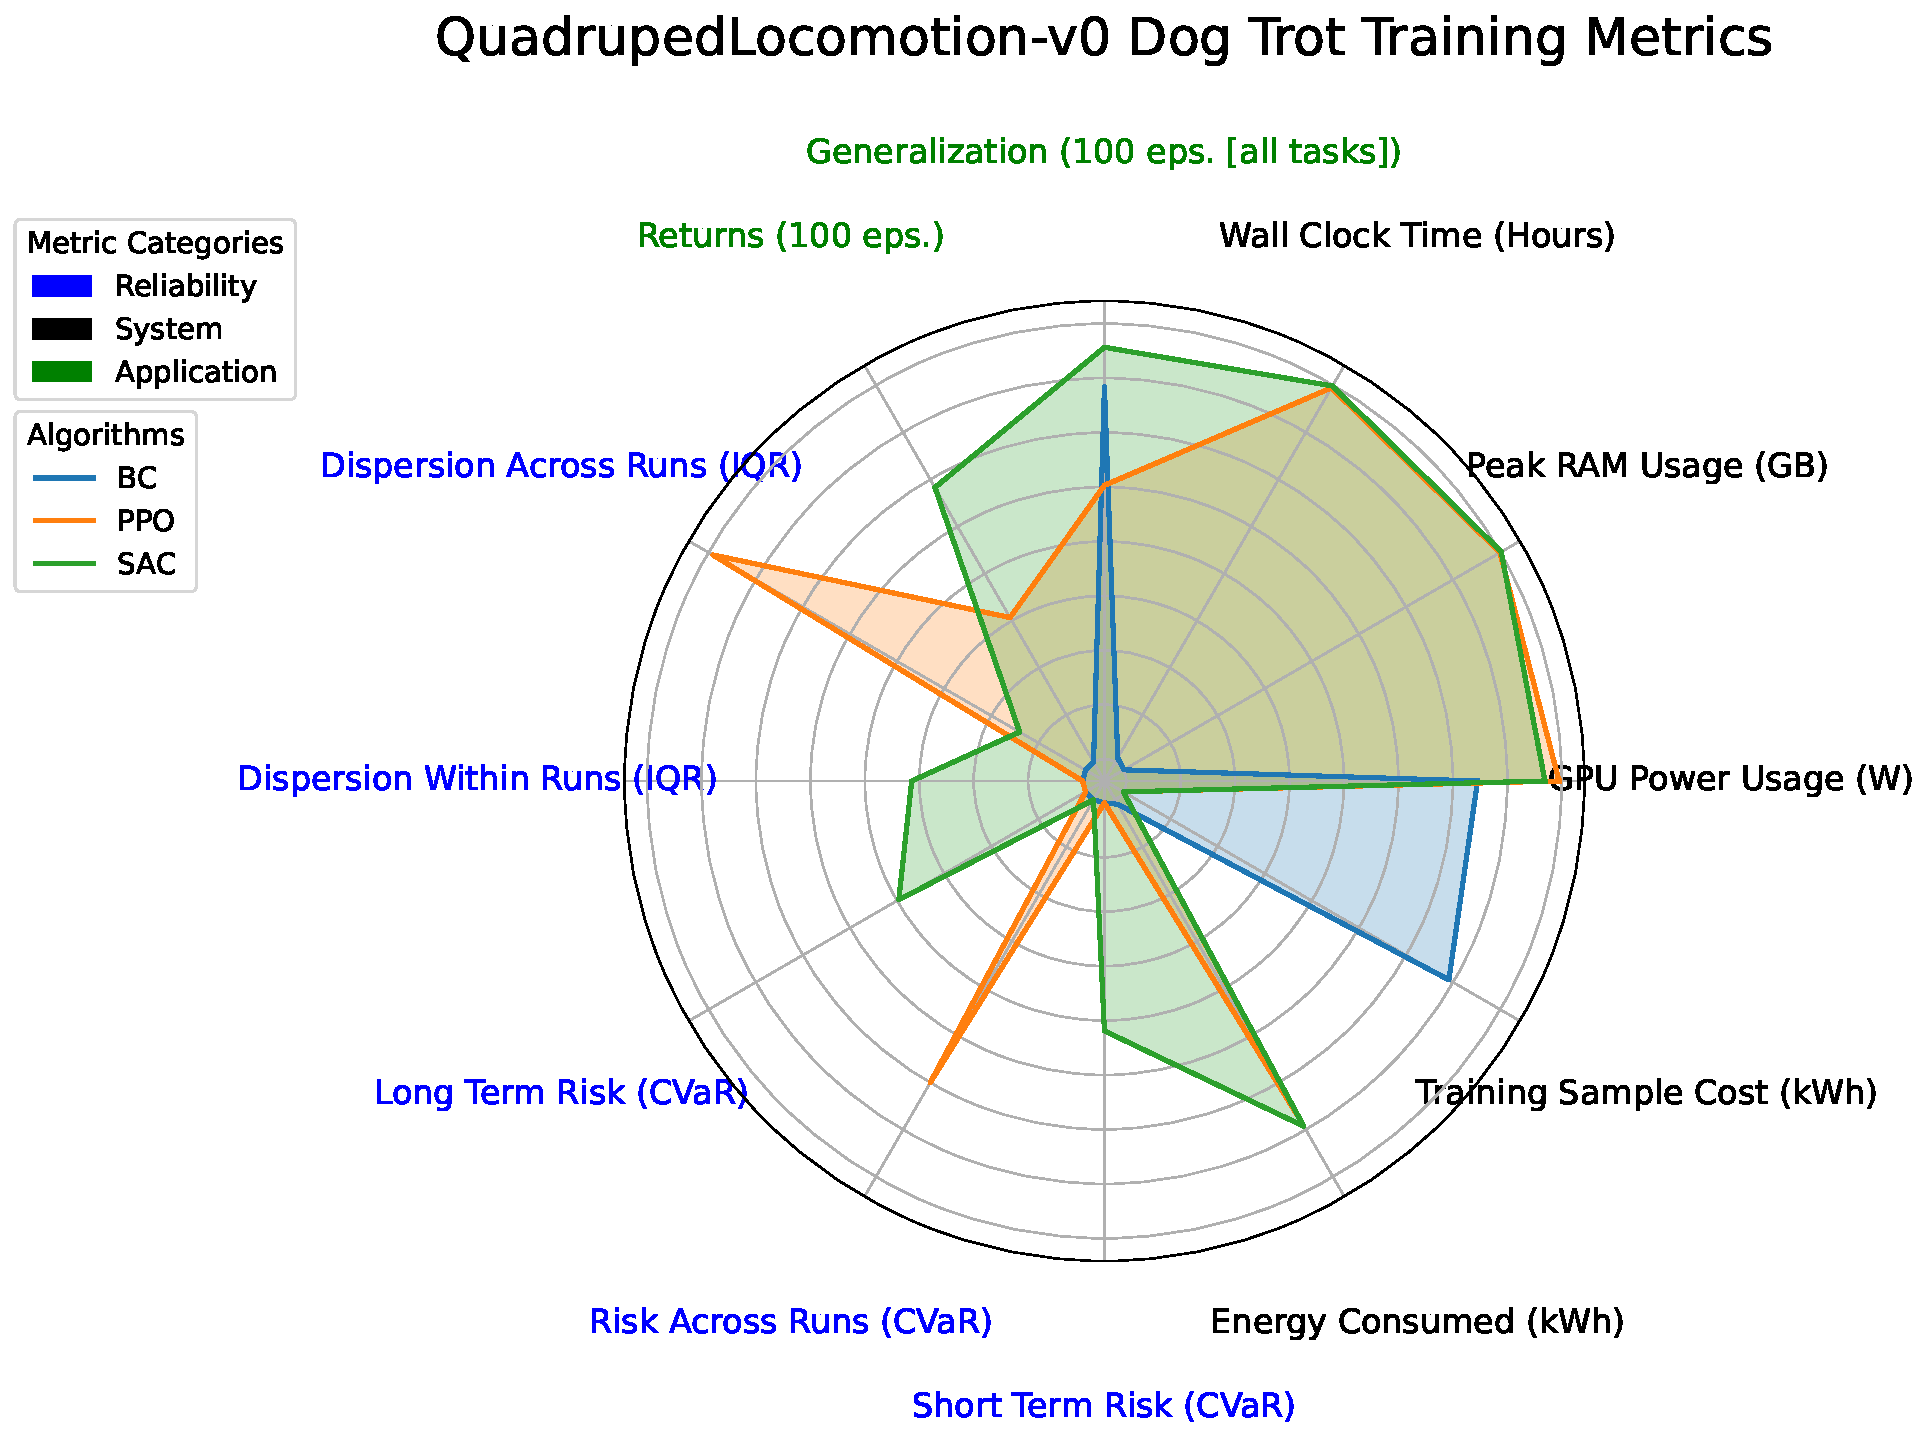
\includegraphics[width=\linewidth]{img/quadruped_locomotion/QuadrupedLocomotion-v0 Dog Trot Training Metrics.pdf}
  \end{minipage}
  \hfill % optional; adds horizontal spacing
  \begin{minipage}[b]{0.4625\linewidth}
    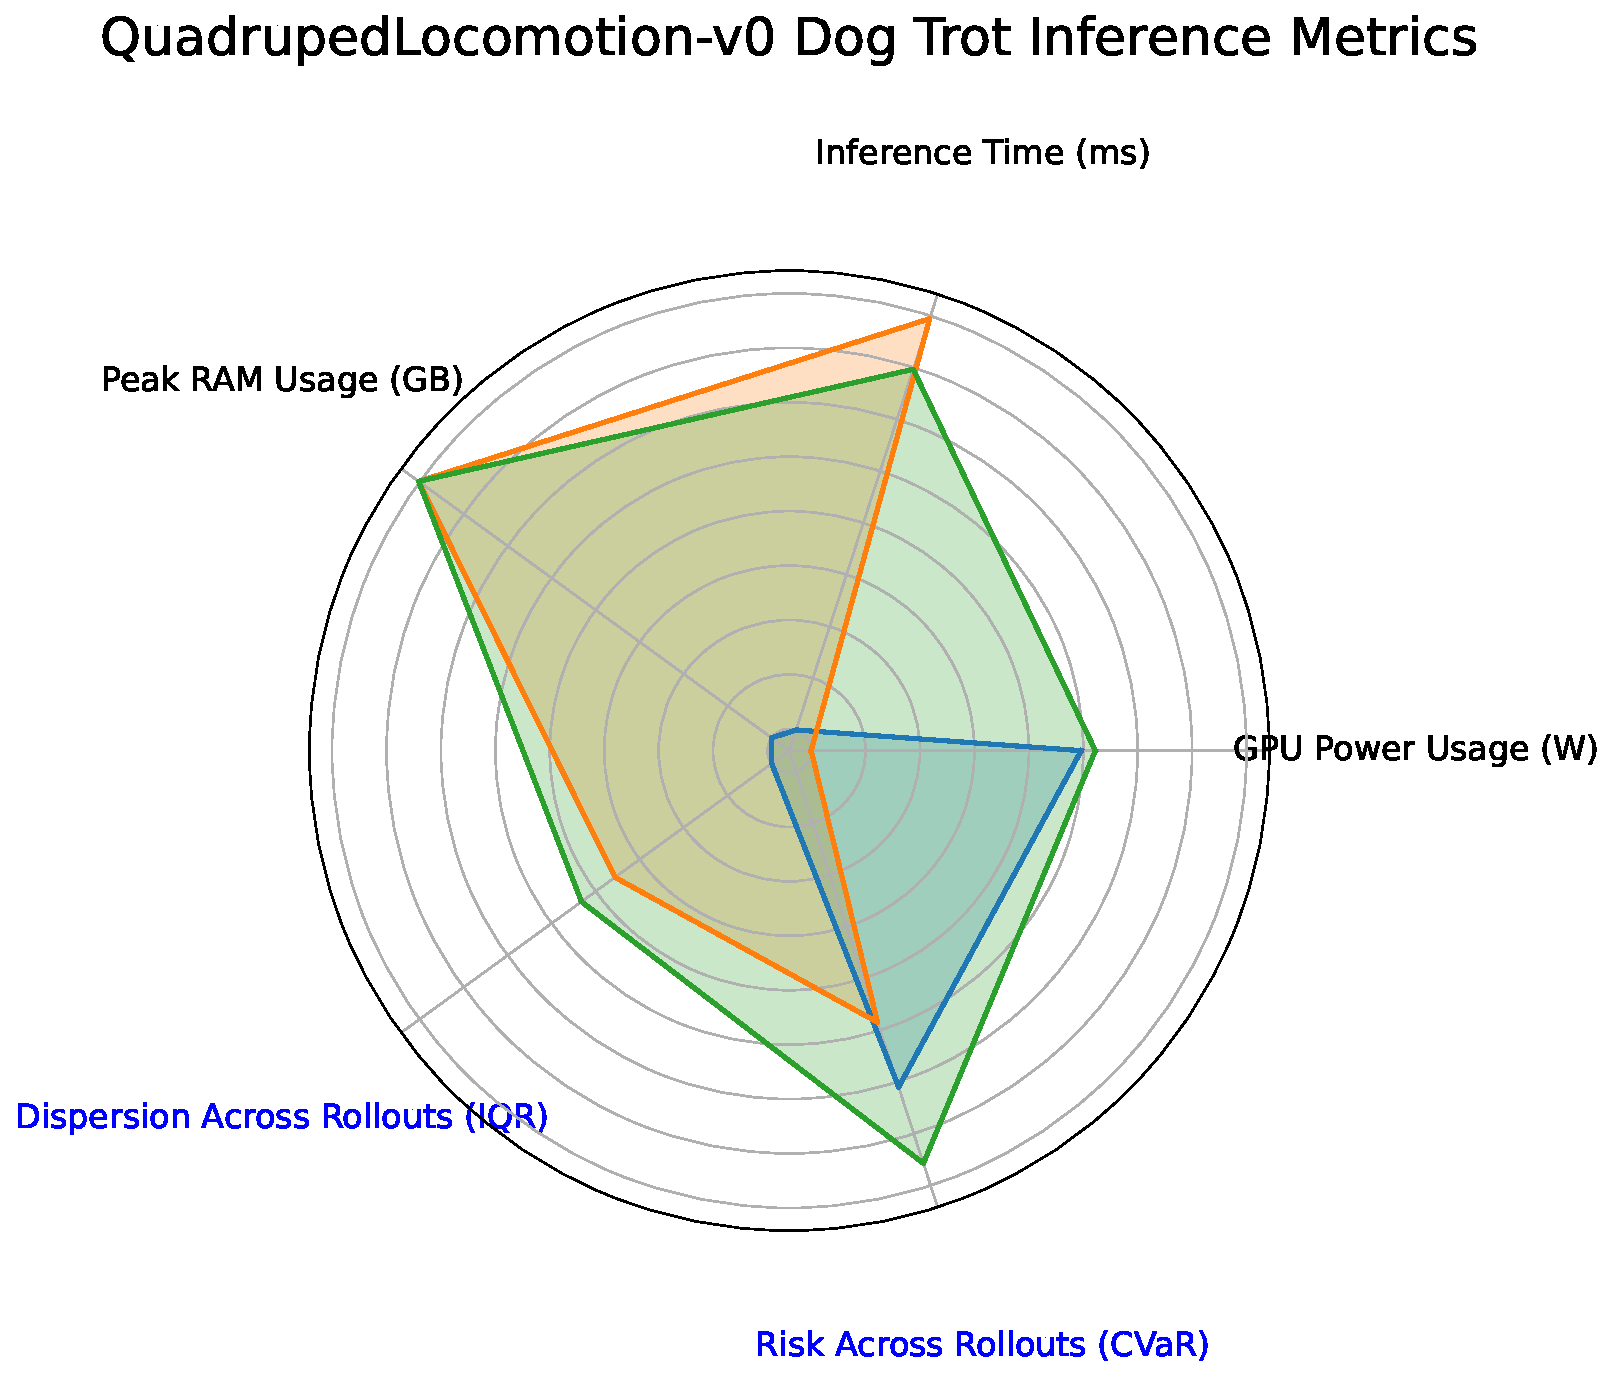
\includegraphics[width=\linewidth]{img/quadruped_locomotion/QuadrupedLocomotion-v0 Dog Trot Inference Metrics.pdf}
  \end{minipage}
  \caption{Graphical representation of metrics for the "dog trot" gait of QuadrupedLocomotion-v0}
  \label{fig:appendix_radar_quadruped_locomotion_dog_trot}
\end{figure}
% ---- Locomotion Pace
\begin{figure}[H]
  \centering
  \begin{minipage}[b]{0.53\linewidth}
    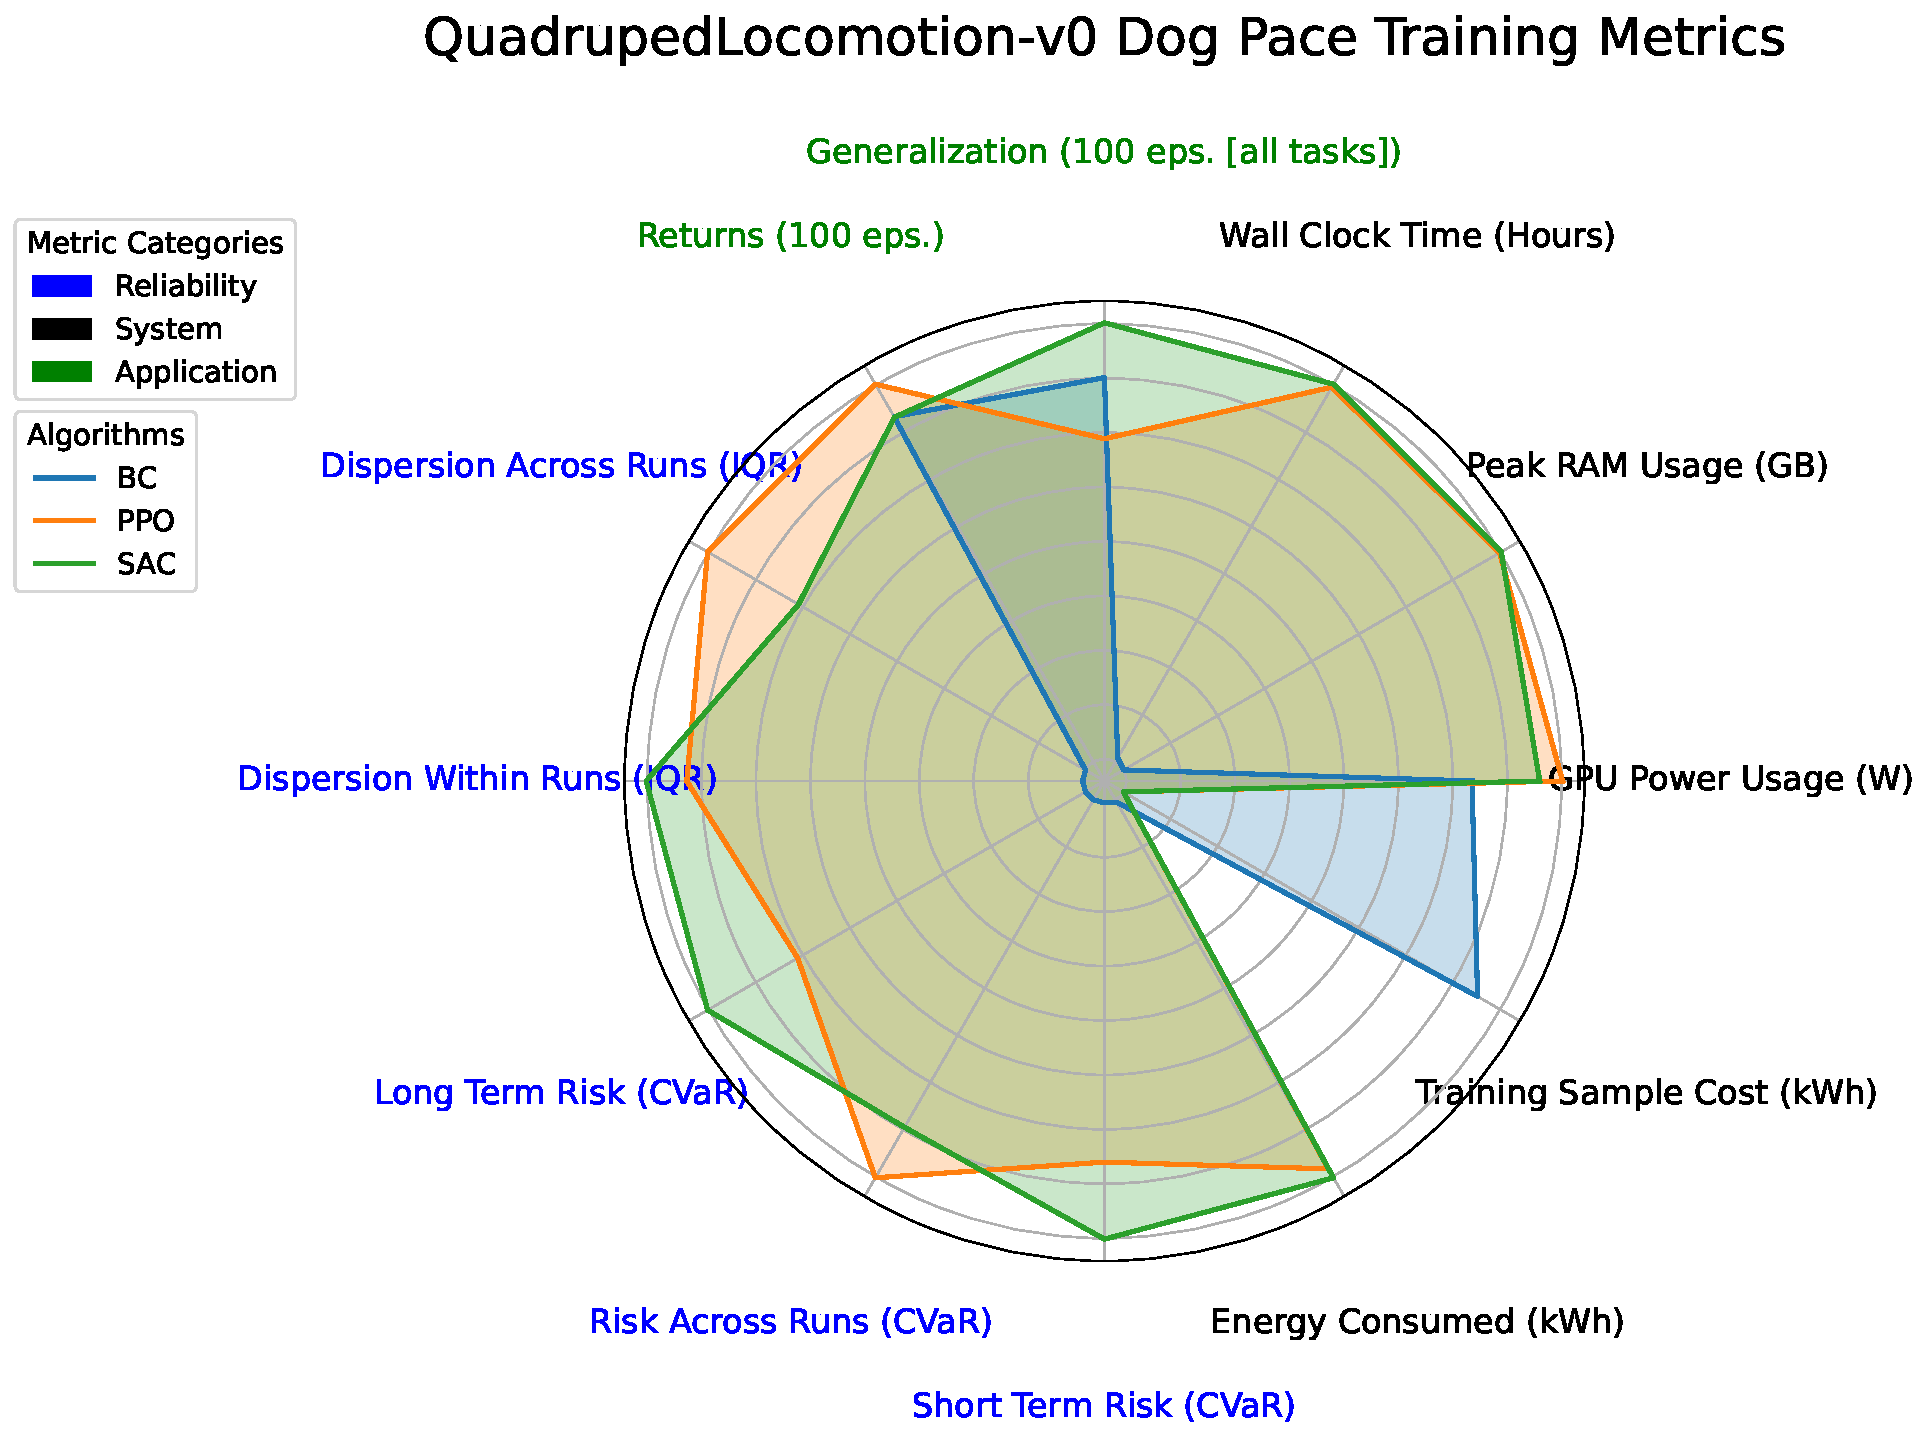
\includegraphics[width=\linewidth]{img/quadruped_locomotion/QuadrupedLocomotion-v0 Dog Pace Training Metrics.pdf}
  \end{minipage}
  \hfill % optional; adds horizontal spacing
  \begin{minipage}[b]{0.4625\linewidth}
    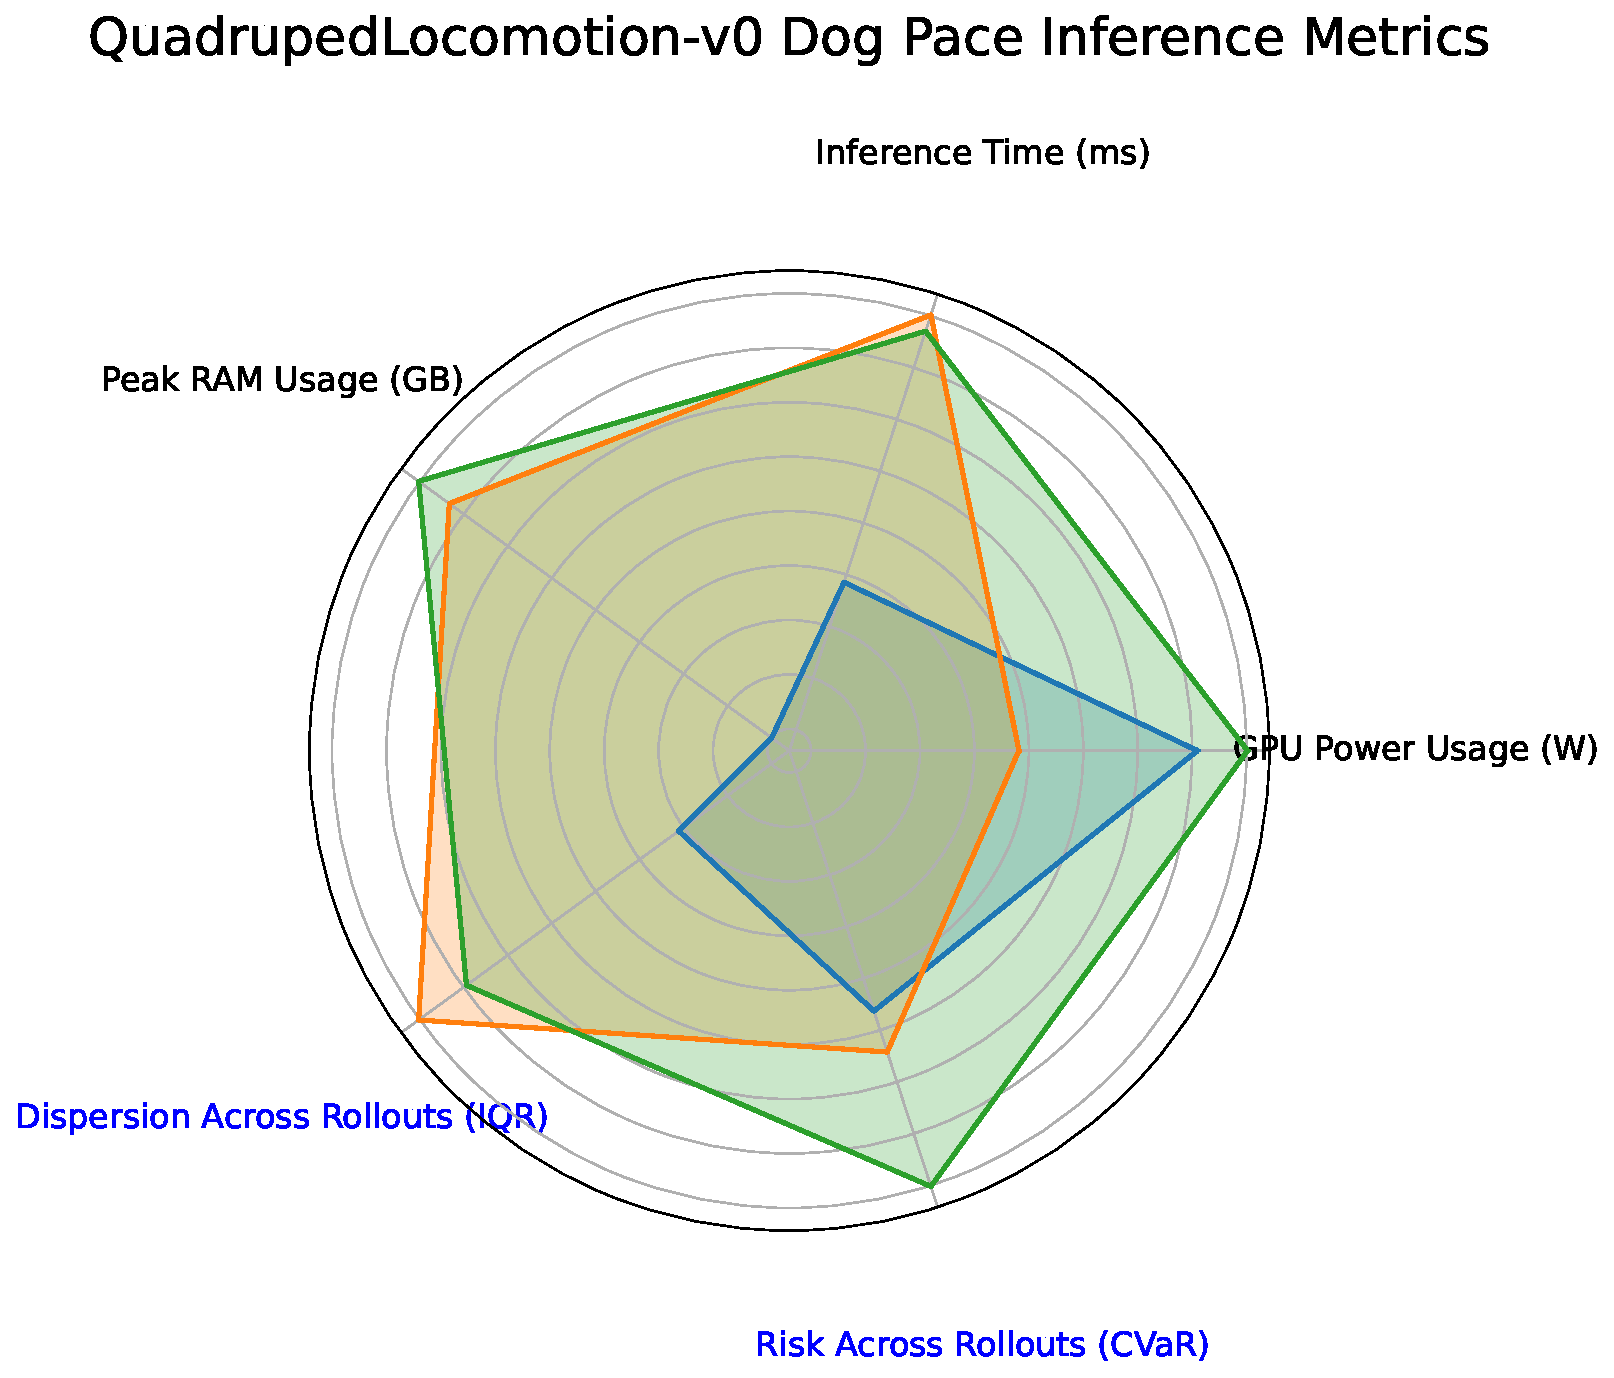
\includegraphics[width=\linewidth]{img/quadruped_locomotion/QuadrupedLocomotion-v0 Dog Pace Inference Metrics.pdf}
  \end{minipage}
  \caption{Graphical representation of metrics for the "dog pace" gait of QuadrupedLocomotion-v0}
  \label{fig:appendix_radar_quadruped_locomotion_dog_pace}
\end{figure}

\newpage

% ---- Circuit Training Toy
\begin{figure}[!htbp]
  \centering
  \begin{minipage}[b]{0.53\linewidth}
    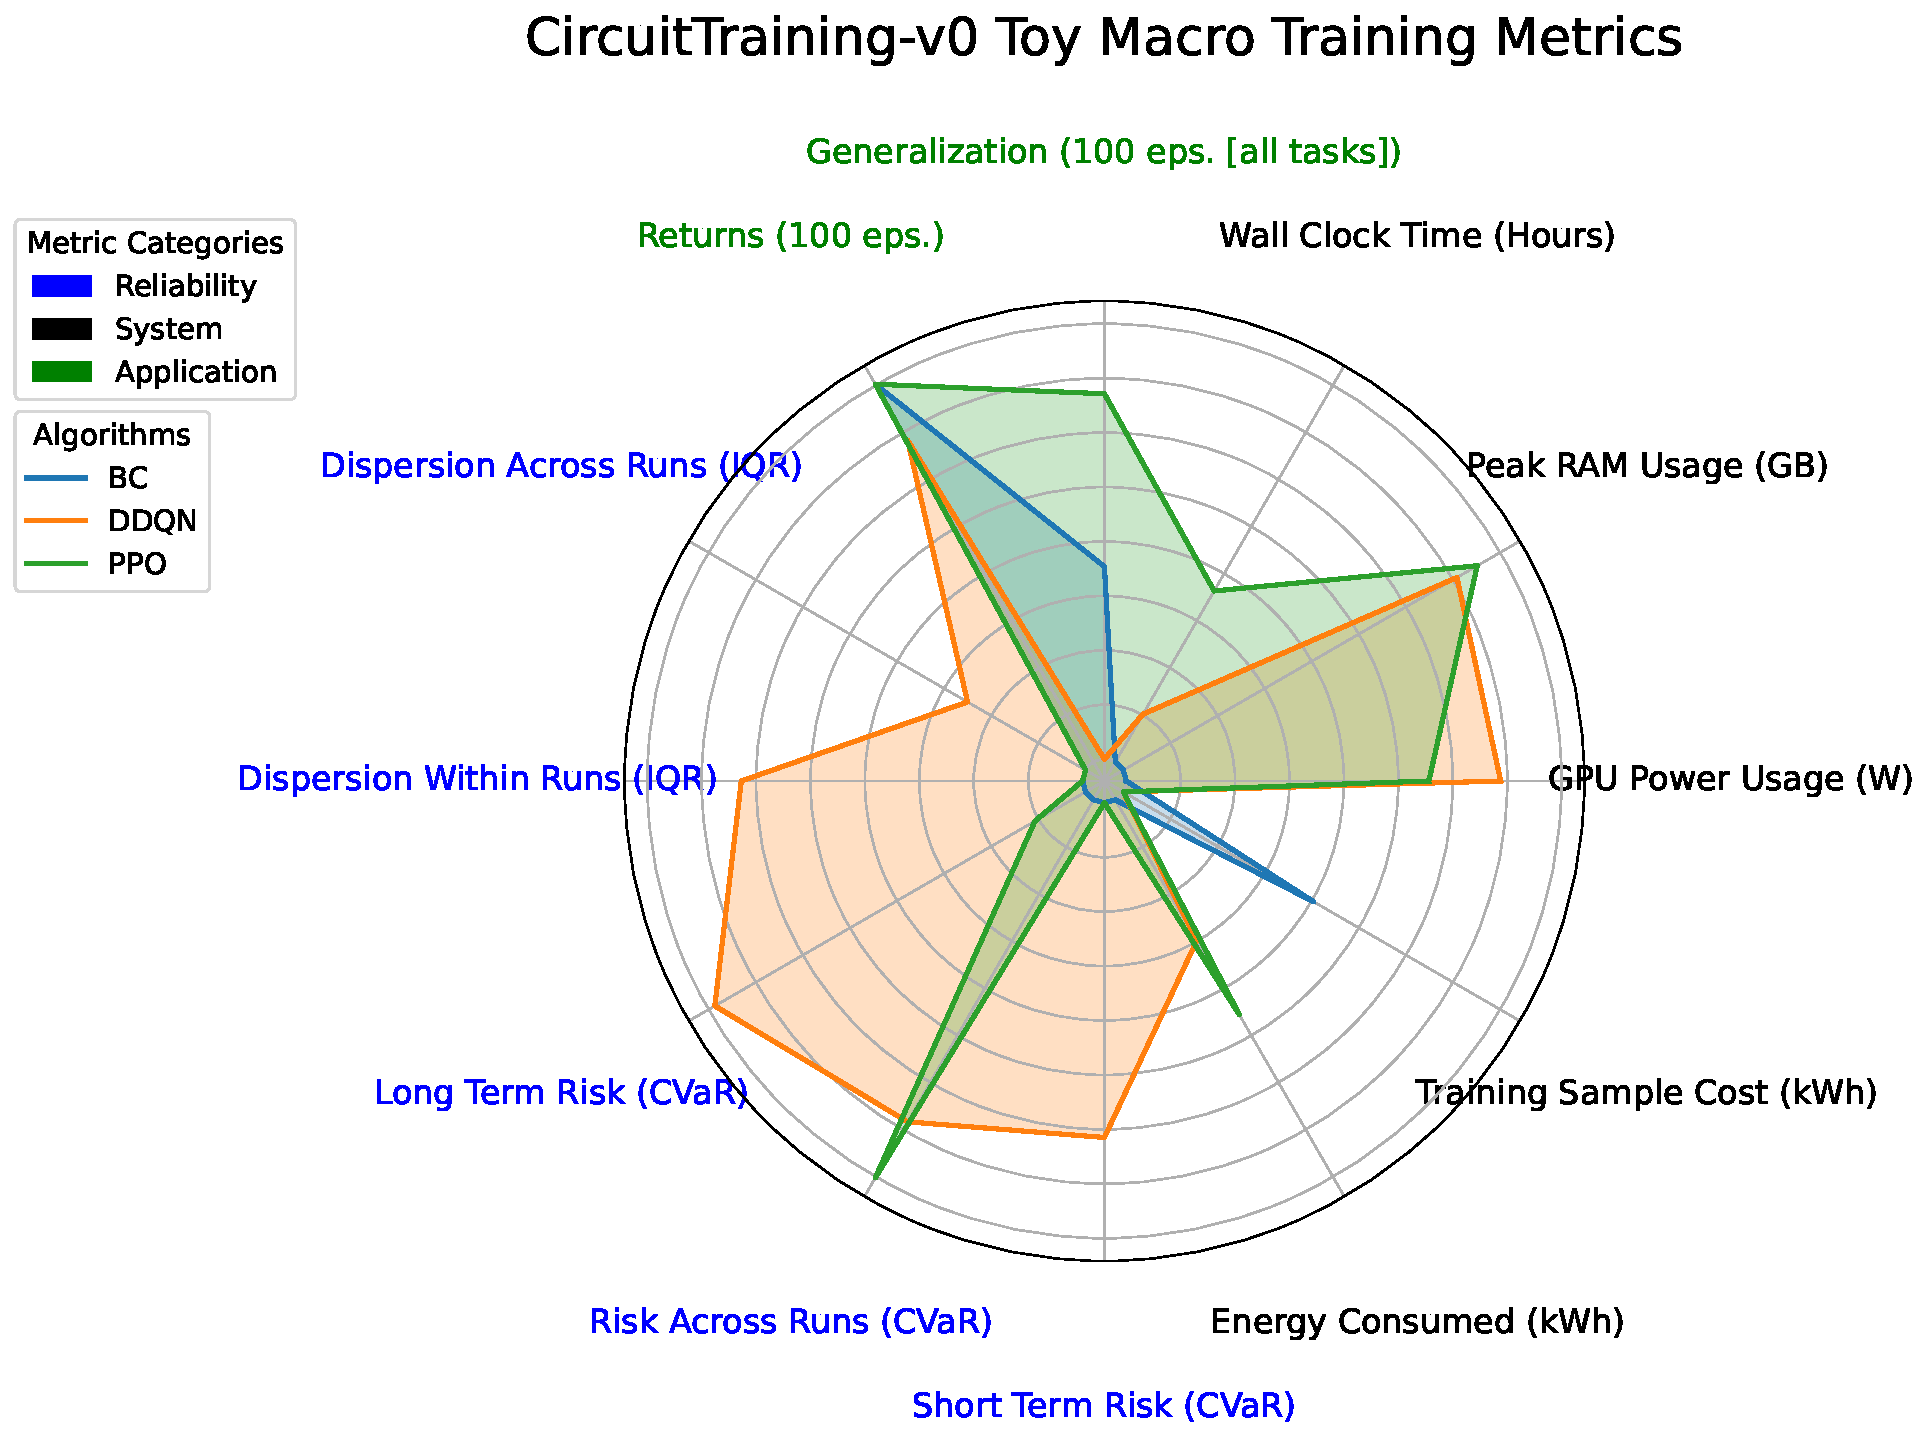
\includegraphics[width=\linewidth]{img/circuit_training/CircuitTraining-v0 Toy Macro Training Metrics.pdf}
  \end{minipage}
  \hfill % optional; adds horizontal spacing
  \begin{minipage}[b]{0.44\linewidth}
    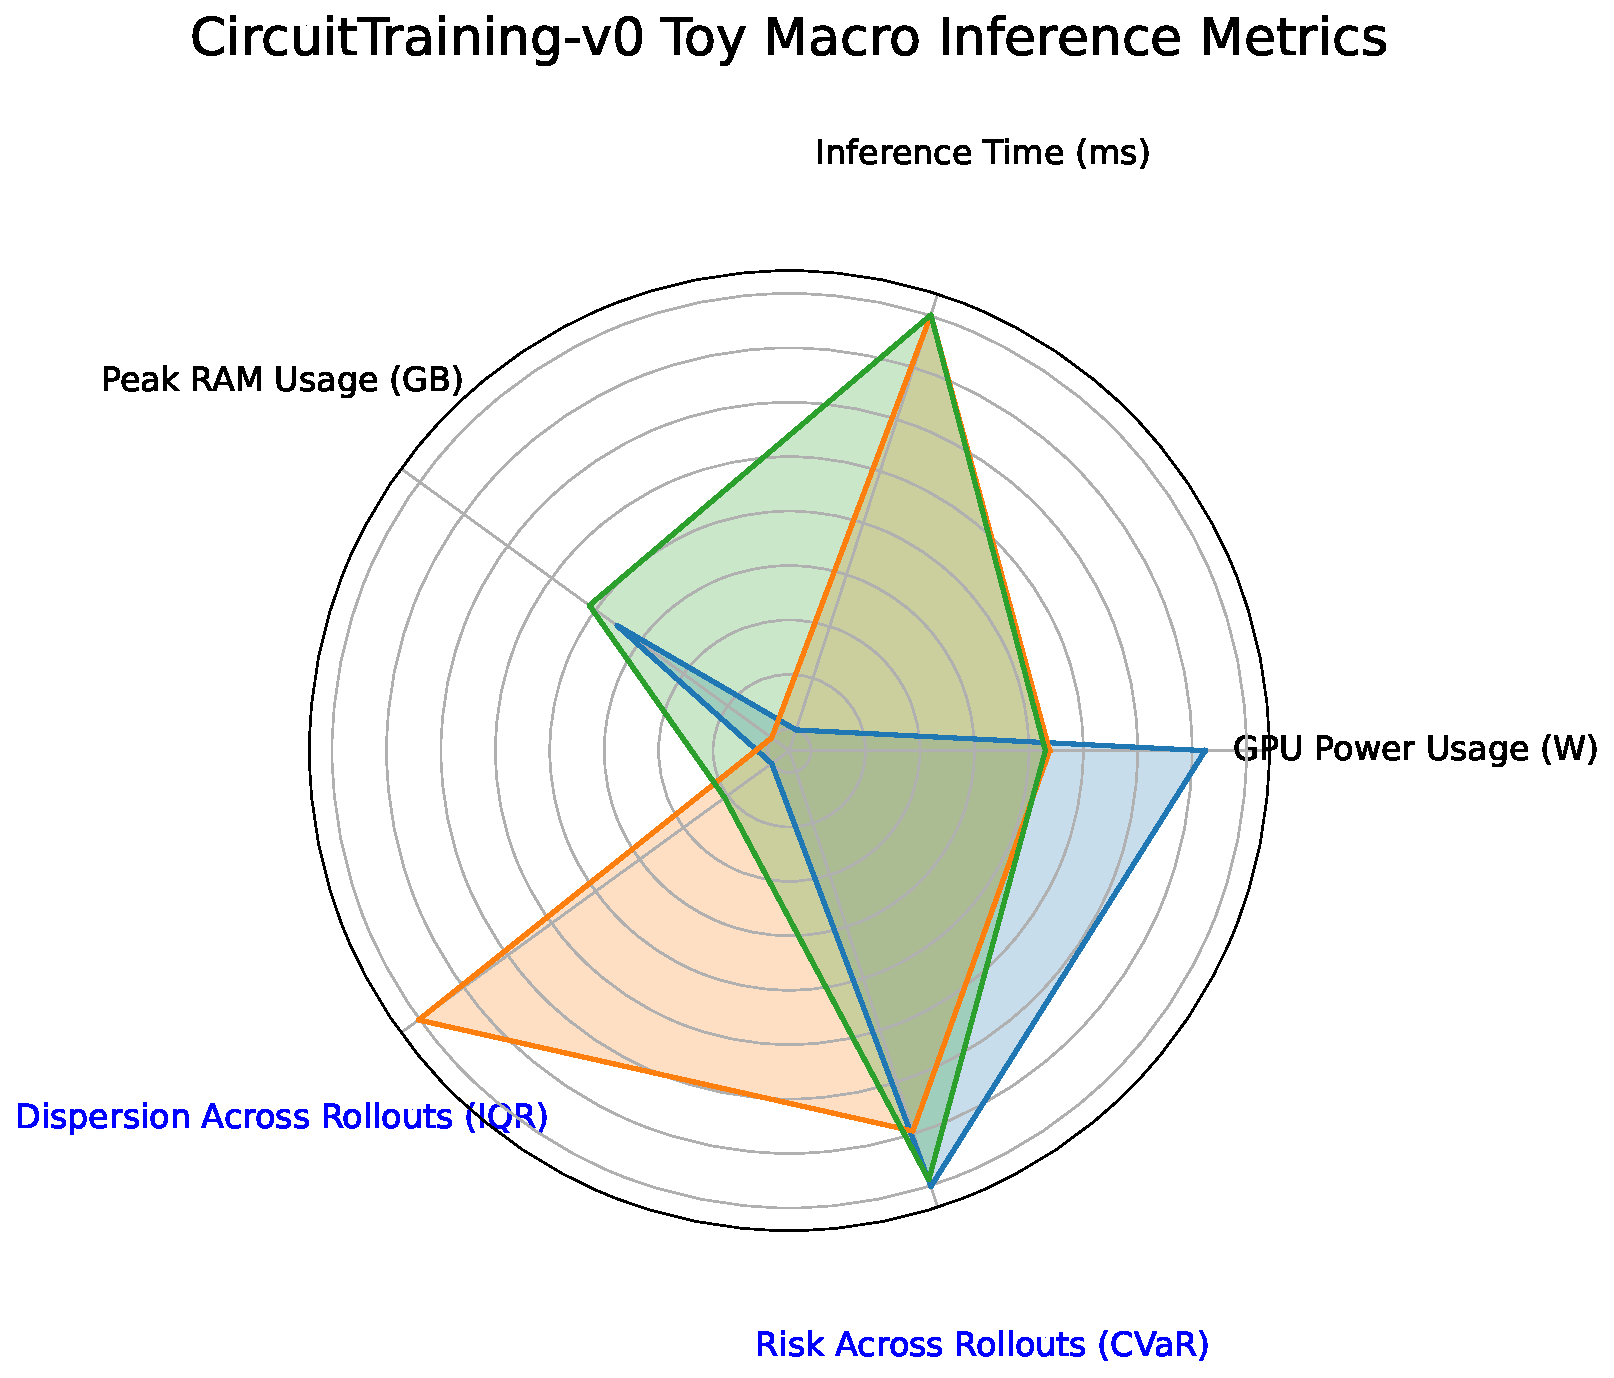
\includegraphics[width=\linewidth]{img/circuit_training/CircuitTraining-v0 Toy Macro Inference Metrics.pdf}
  \end{minipage}
  \caption{Graphical representation of metrics for the "Toy Macro" netlist task of CircuitTraining-v0}
  \label{fig:appendix_circuit_training_toy_macro}
\end{figure}


% ---- Circuit Training Ariane
\begin{figure}[!htbp]
  \centering
  \begin{minipage}[b]{0.53\linewidth}
    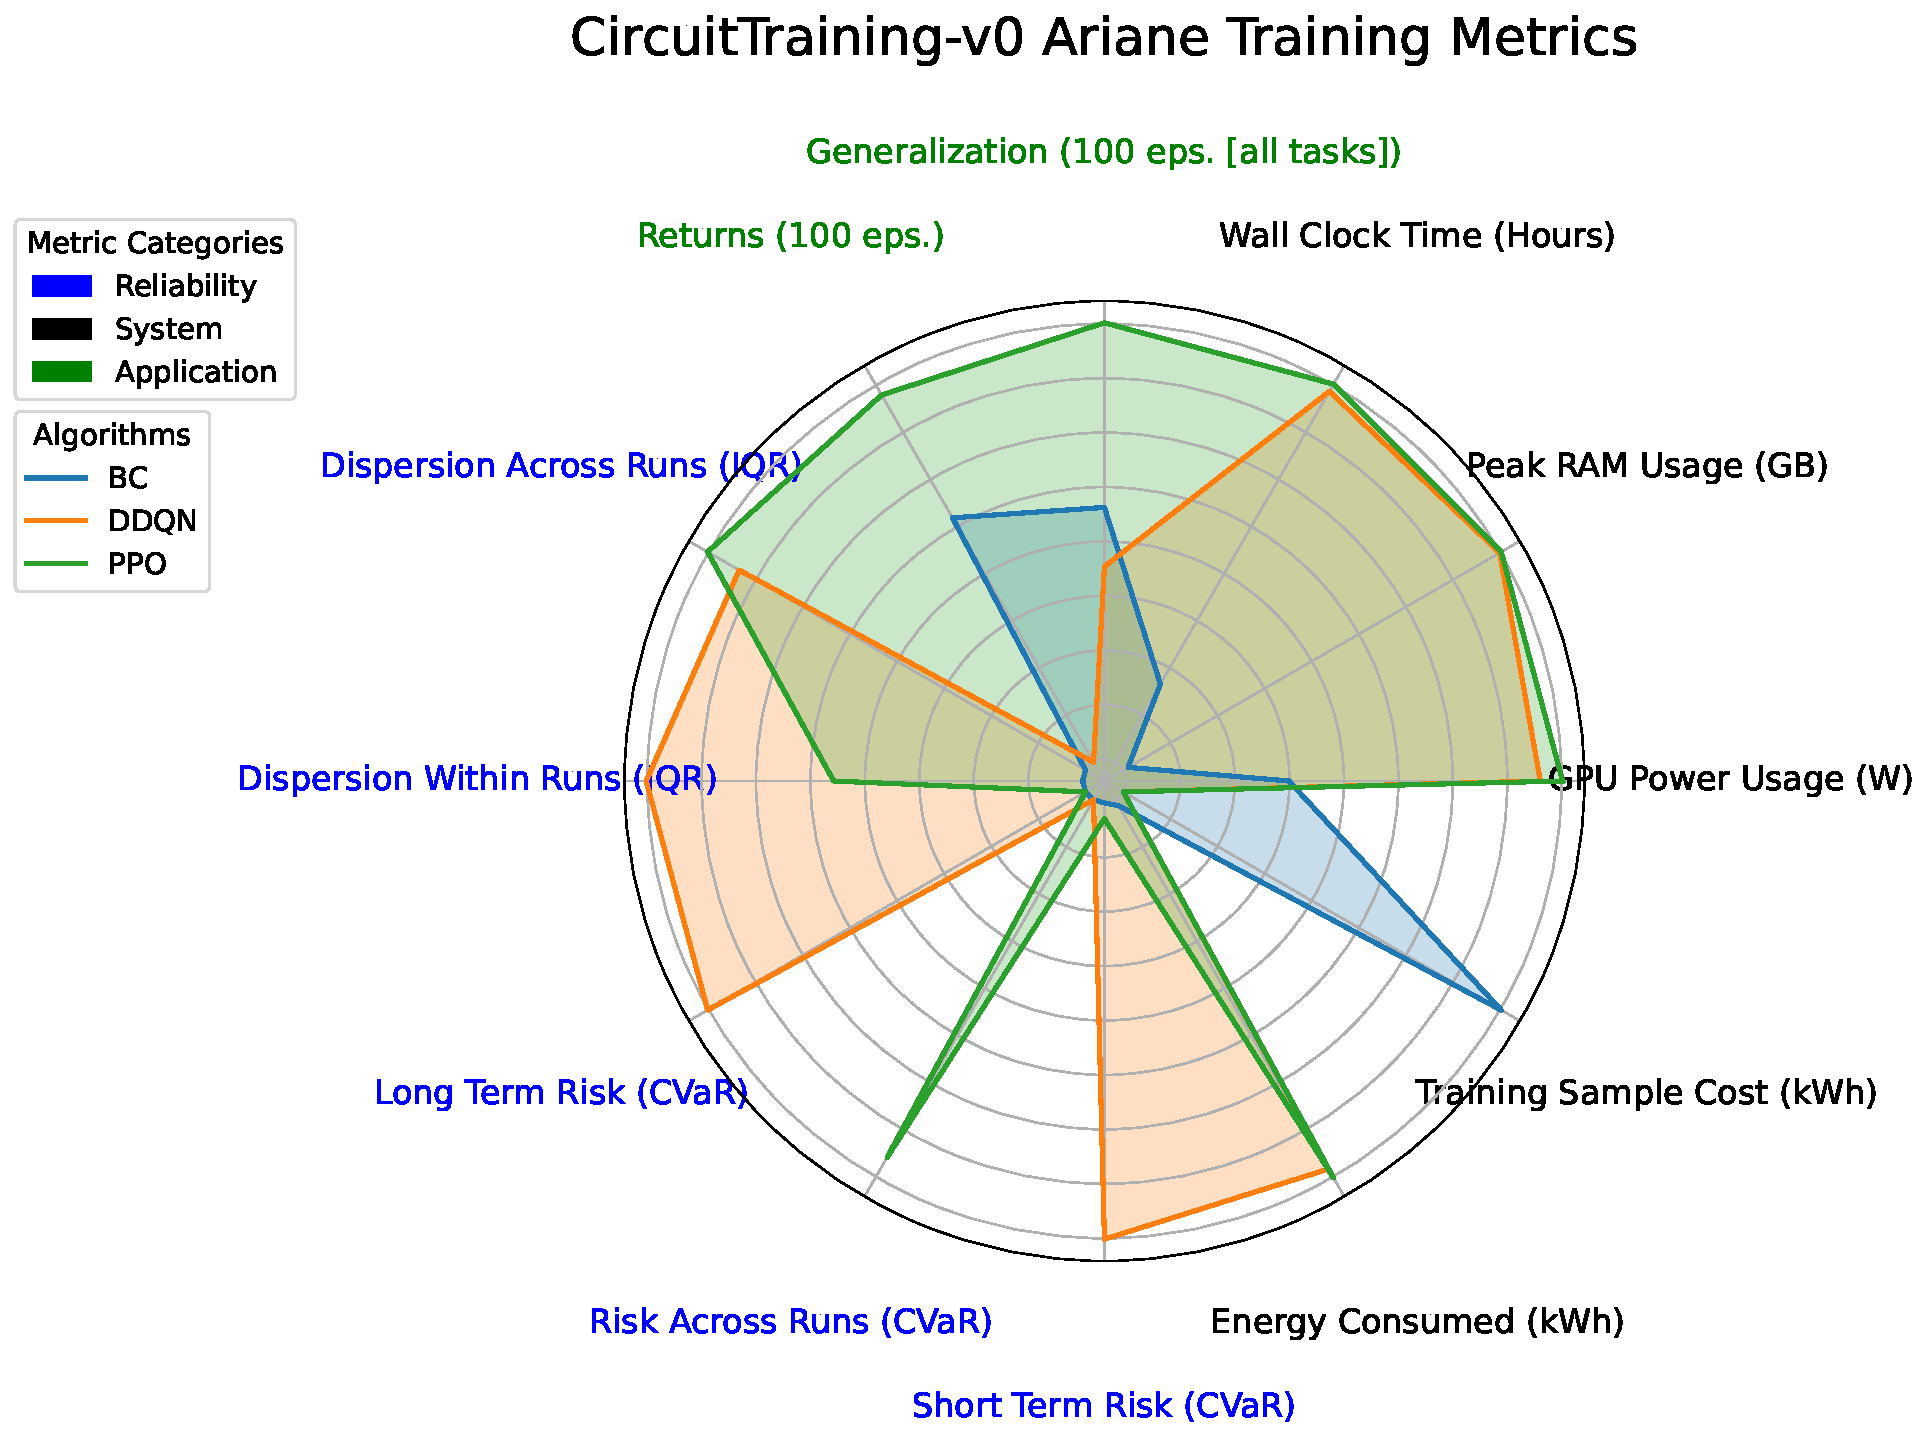
\includegraphics[width=\linewidth]{img/circuit_training/CircuitTraining-v0 Ariane Training Metrics.pdf}
  \end{minipage}
  \hfill % optional; adds horizontal spacing
  \begin{minipage}[b]{0.44\linewidth}
    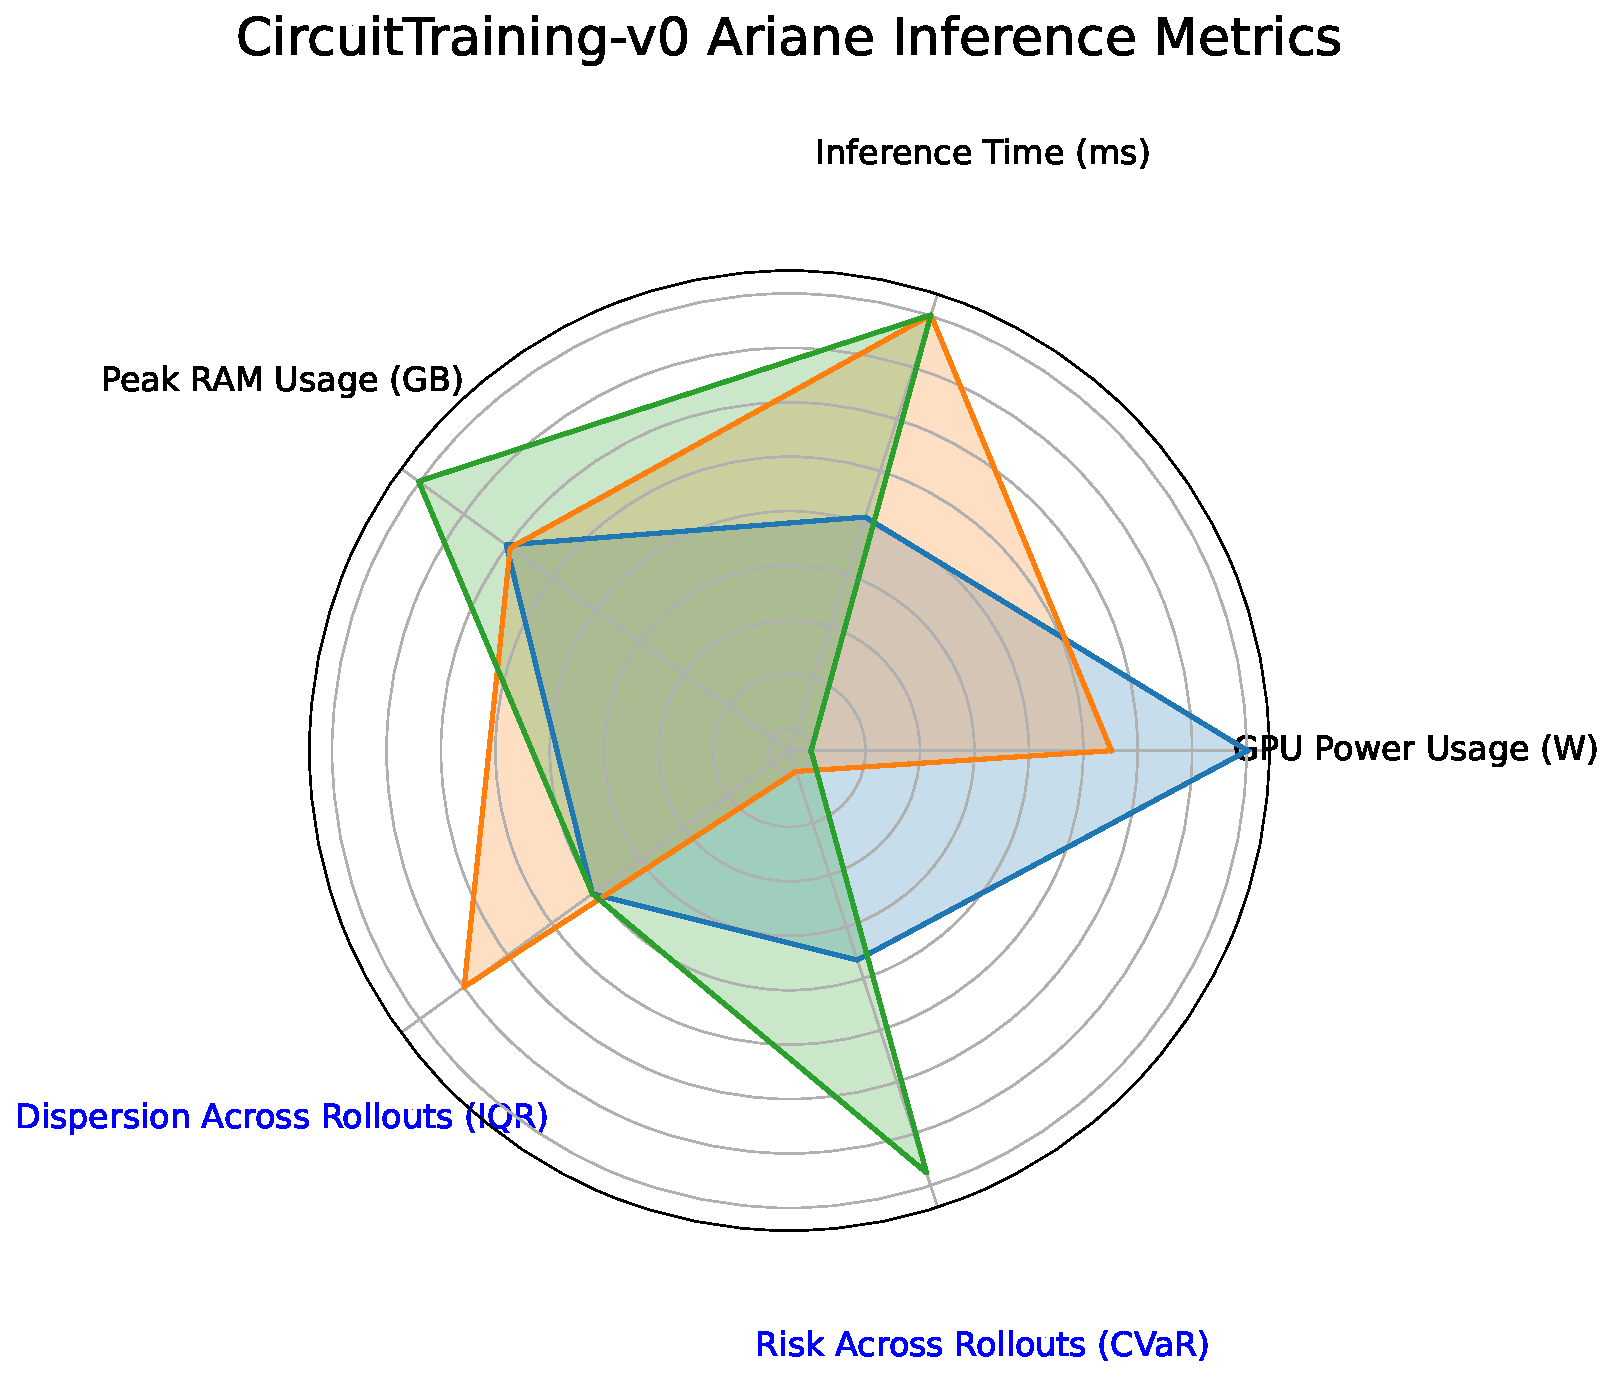
\includegraphics[width=\linewidth]{img/circuit_training/CircuitTraining-v0 Ariane Inference Metrics.pdf}
  \end{minipage}
  \caption{Graphical representation of metrics for the "Ariane" netlist task of CircuitTraining-v0}
  \label{fig:appendix_circuit_training_ariane}
\end{figure}
\newpage


% ---- WebNav 1 Website
\begin{figure}[!htbp]
  \centering
  \begin{minipage}[b]{0.53\linewidth}
    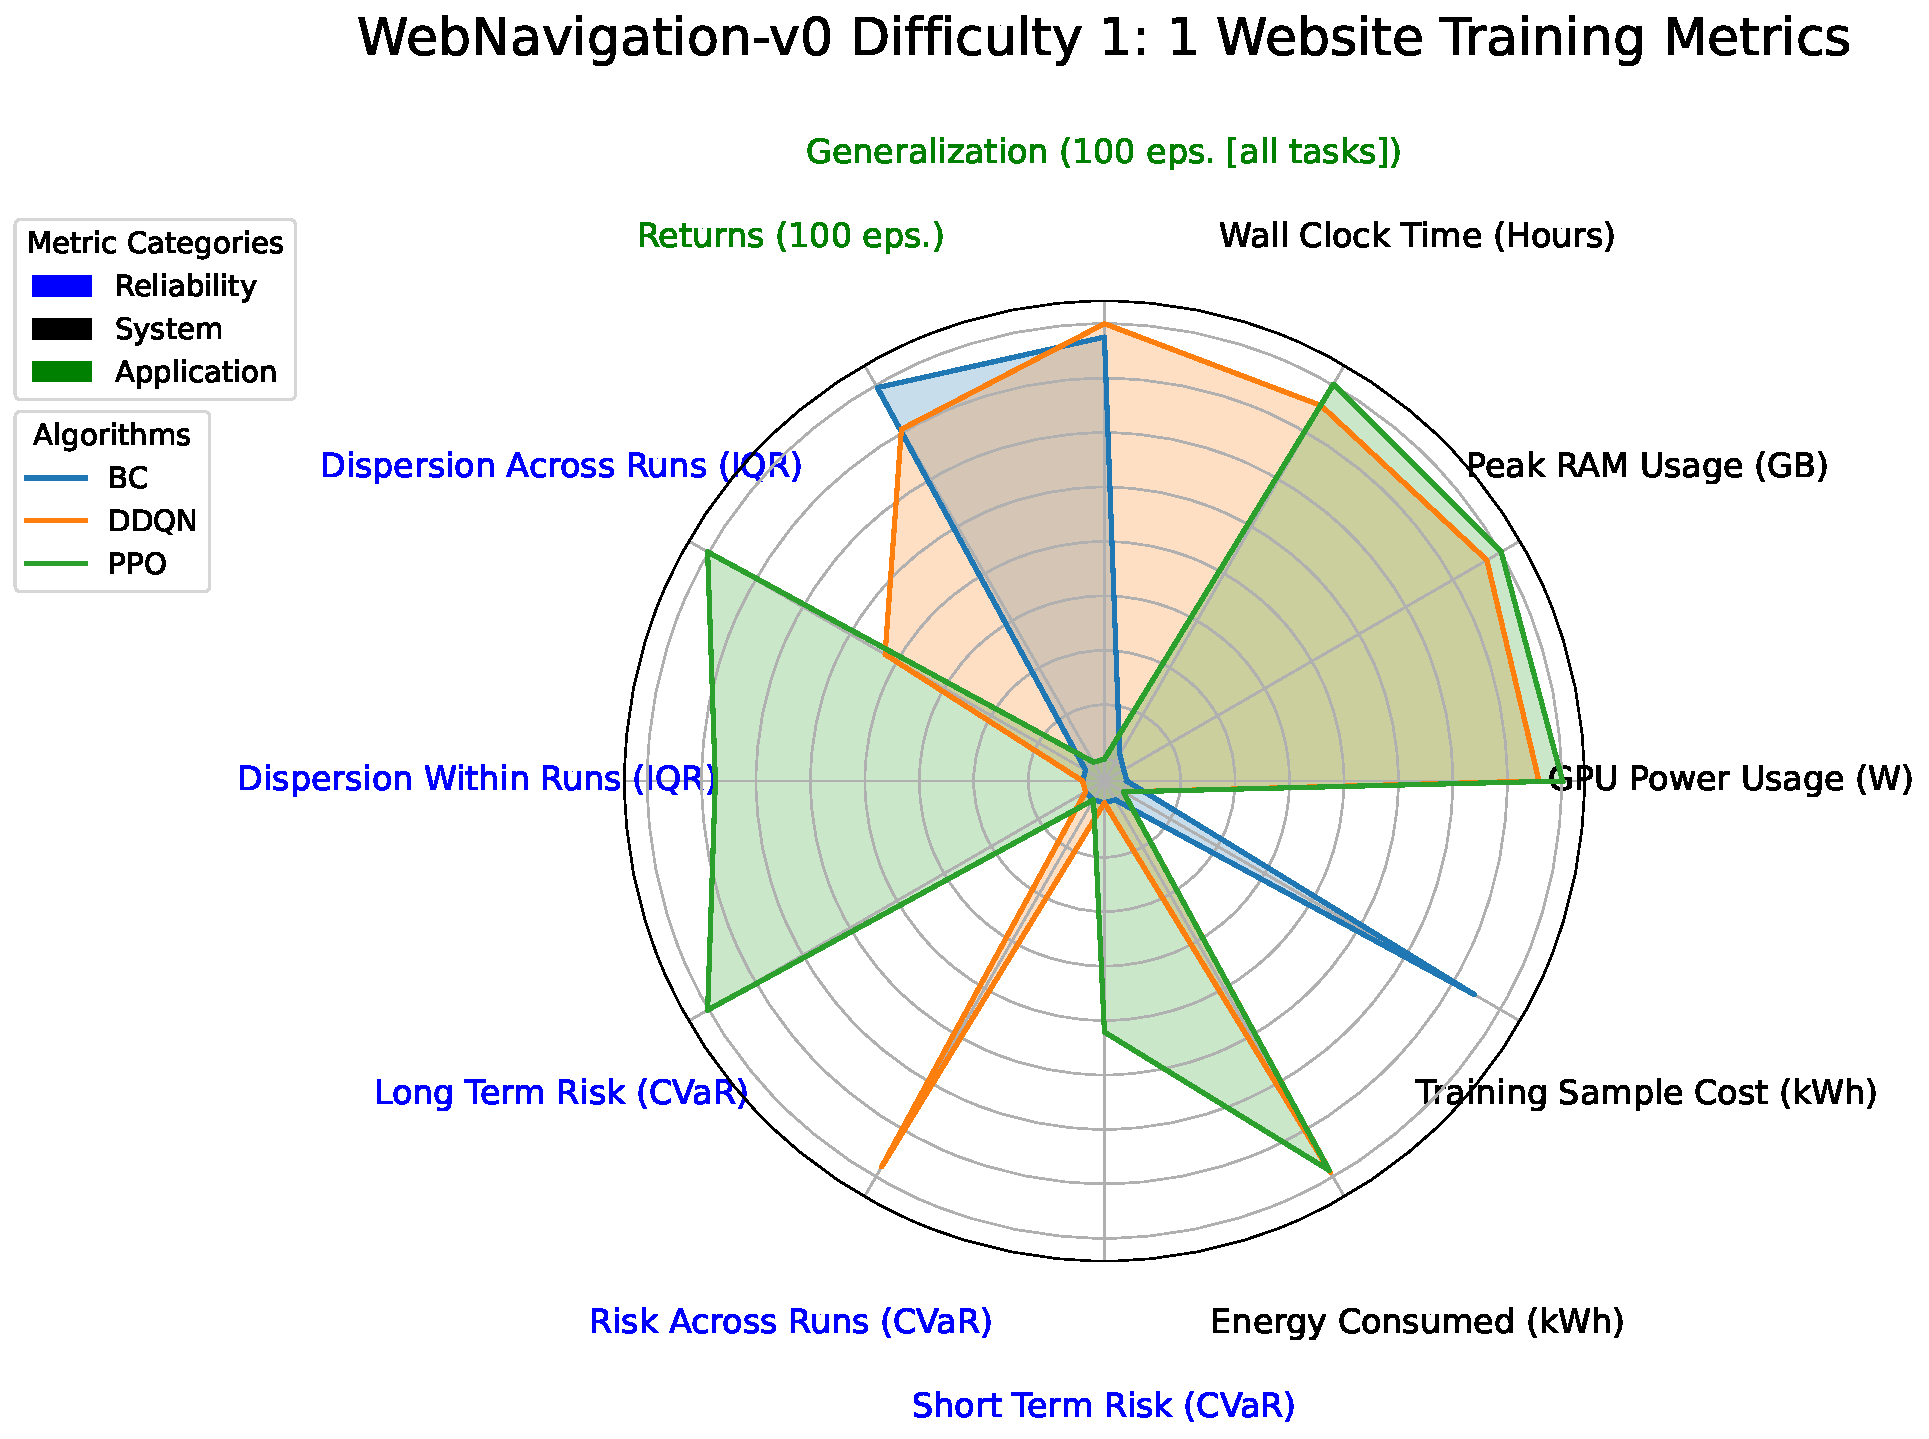
\includegraphics[width=\linewidth]{img/web_nav/WebNavigation-v0 Difficulty 1_ 1 Website Training Metrics.pdf}
  \end{minipage}
  \hfill % optional; adds horizontal spacing
  \begin{minipage}[b]{0.4625\linewidth}
    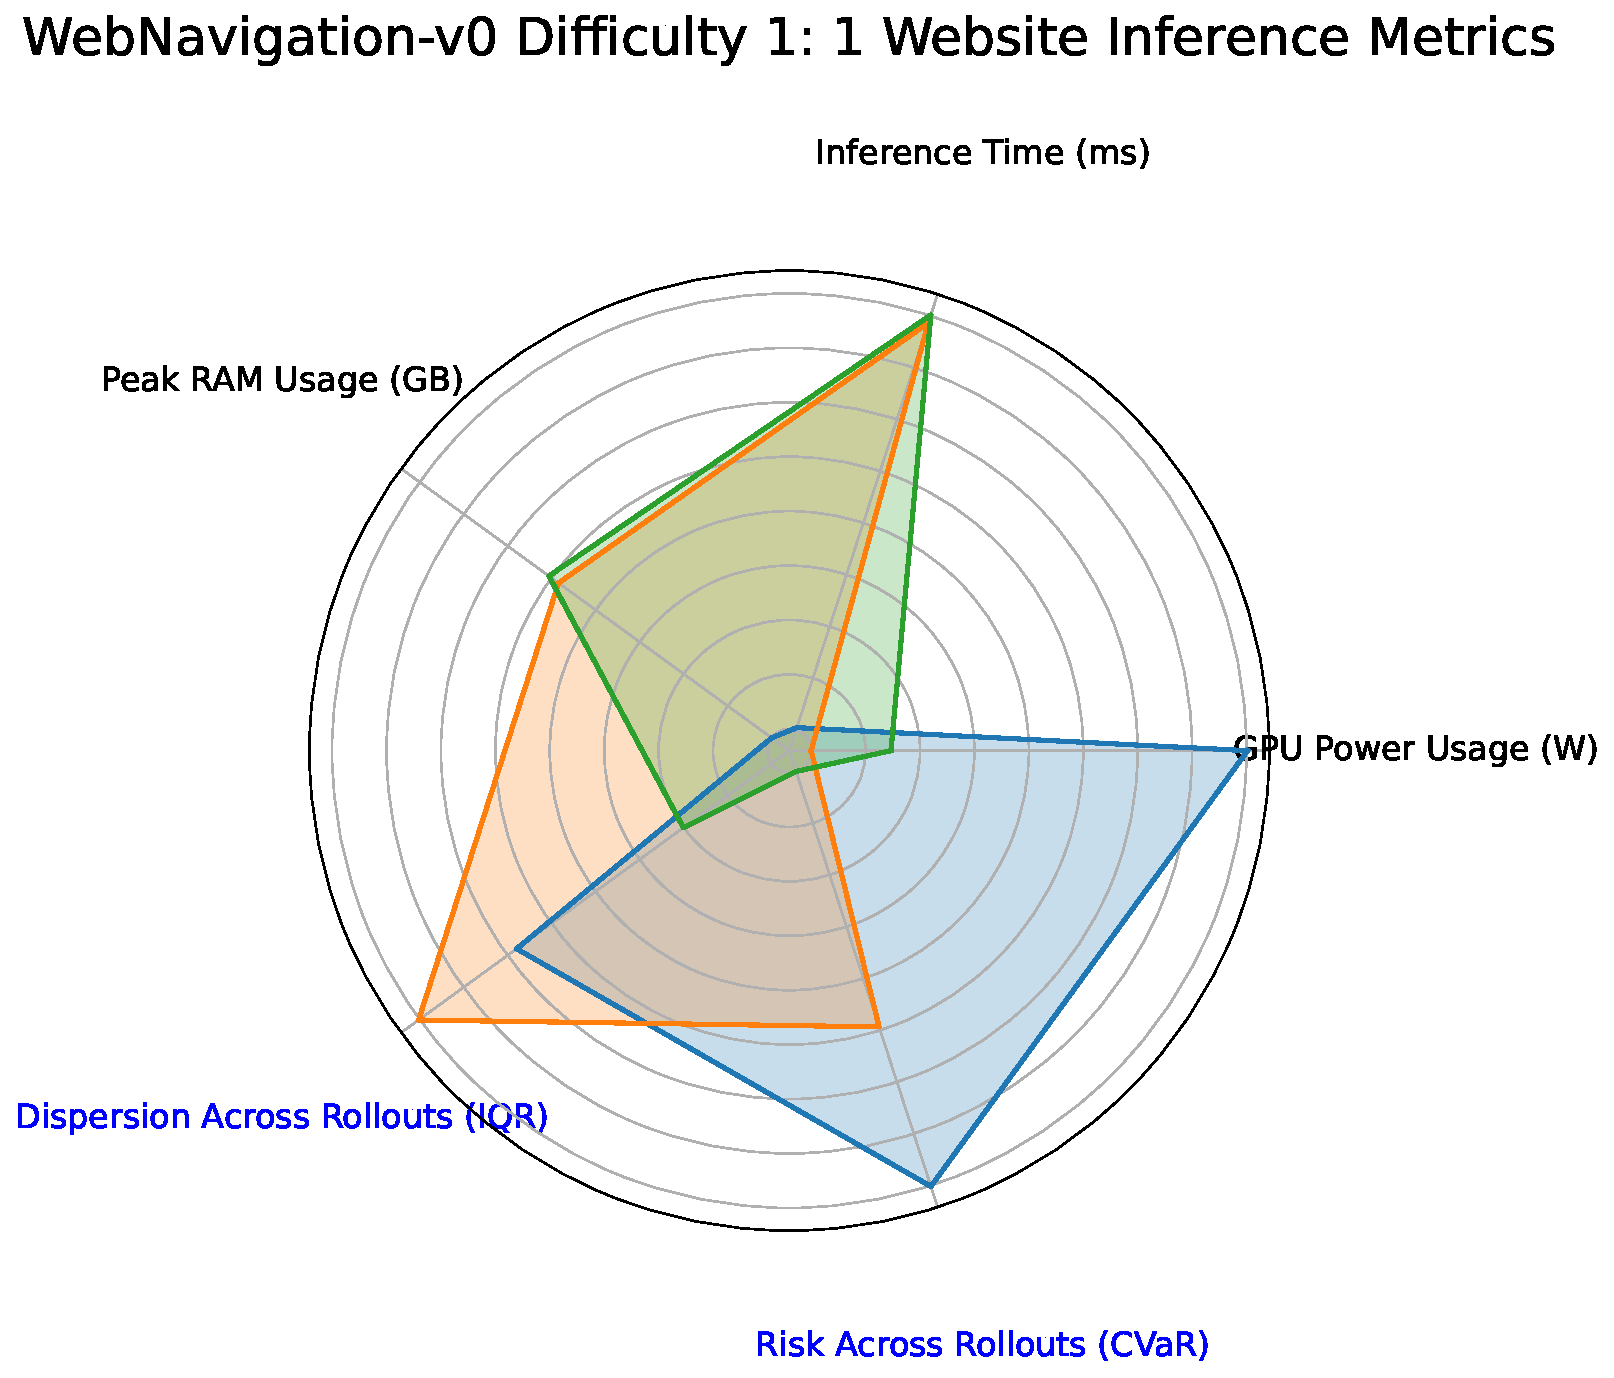
\includegraphics[width=\linewidth]{img/web_nav/WebNavigation-v0 Difficulty 1_ 1 Website Inference Metrics.pdf}
  \end{minipage}
  \caption{Graphical representation of metrics for the "difficulty 1, 1 website" task of WebNavigation-v0}
  \label{fig:appendix_radar_web_nav_difficulty1_1website}
\end{figure}


% ---- WebNav 5 Websites
\begin{figure}[!htbp]
  \centering
  \begin{minipage}[b]{0.53\linewidth}
    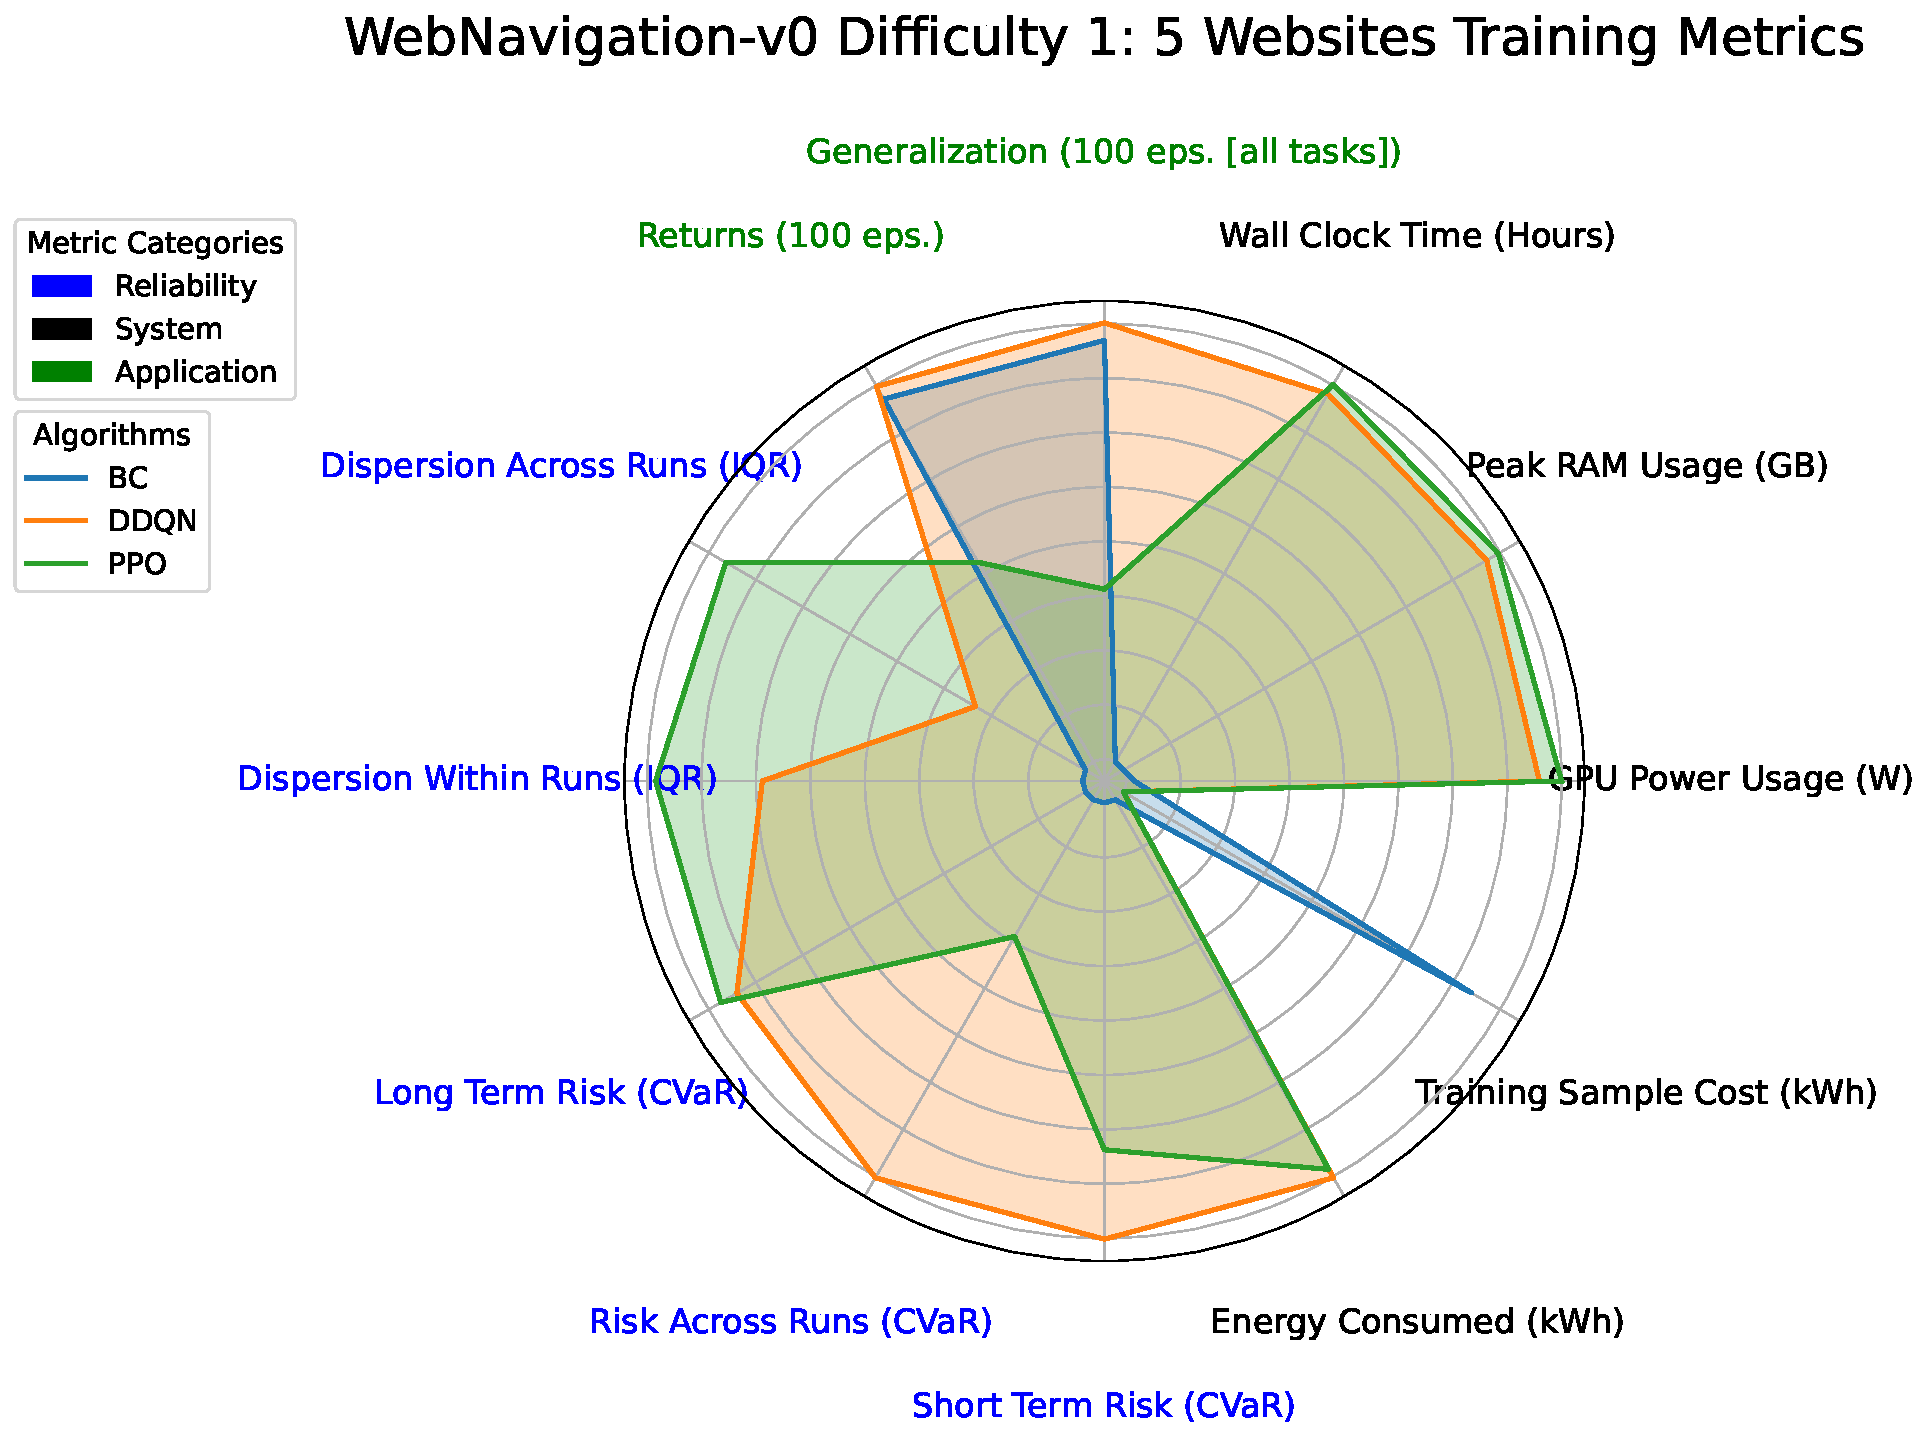
\includegraphics[width=\linewidth]{img/web_nav/WebNavigation-v0 Difficulty 1_ 5 Websites Training Metrics.pdf}
  \end{minipage}
  \hfill % optional; adds horizontal spacing
  \begin{minipage}[b]{0.4625\linewidth}
    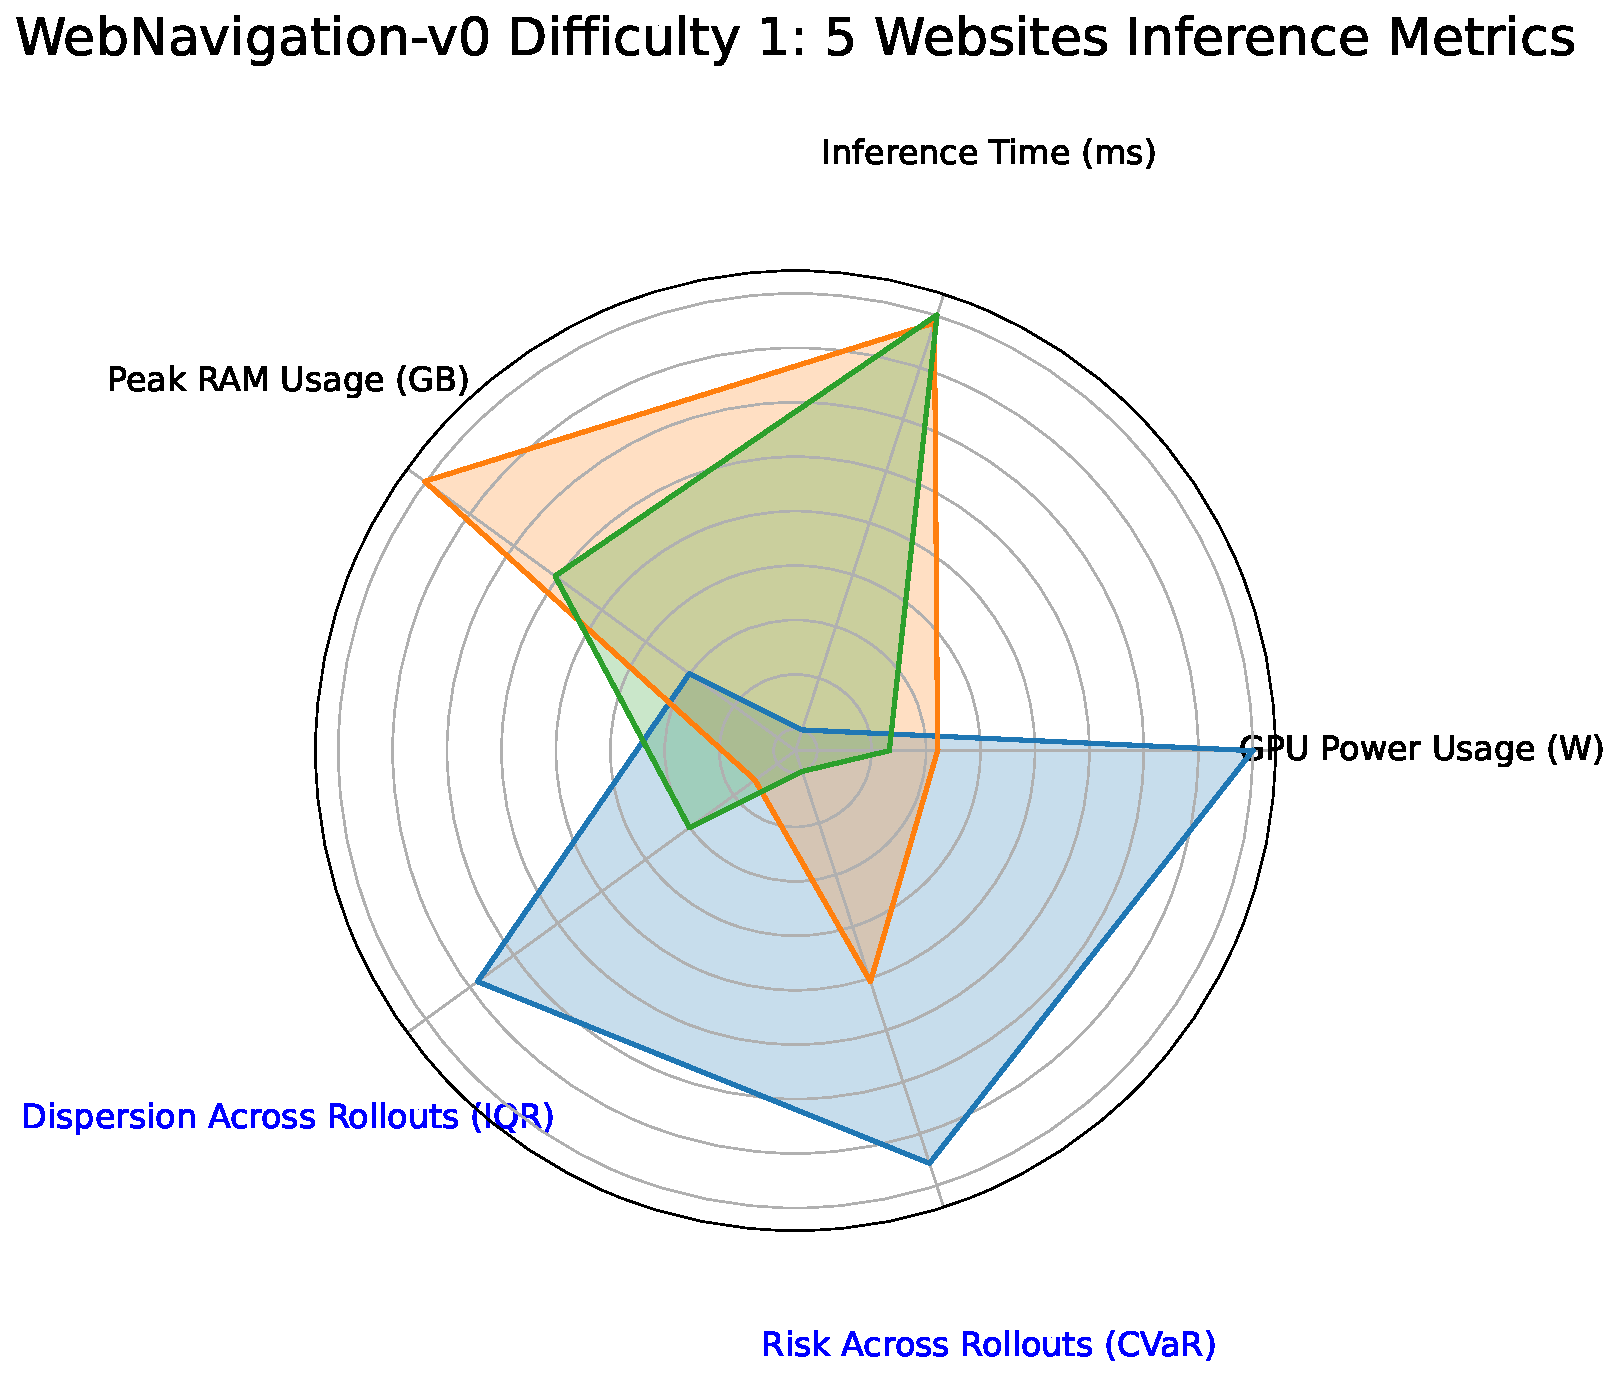
\includegraphics[width=\linewidth]{img/web_nav/WebNavigation-v0 Difficulty 1_ 5 Websites Inference Metrics.pdf}
  \end{minipage}
  \caption{Graphical representation of metrics for the "difficulty 1, 5 websites" task of WebNavigation-v0}
  \label{fig:appendix_radar_web_nav_difficulty1_5websites}
\end{figure}


% ---- WebNav 10 Websites
\begin{figure}[!htbp]
  \centering
  \begin{minipage}[b]{0.53\linewidth}
    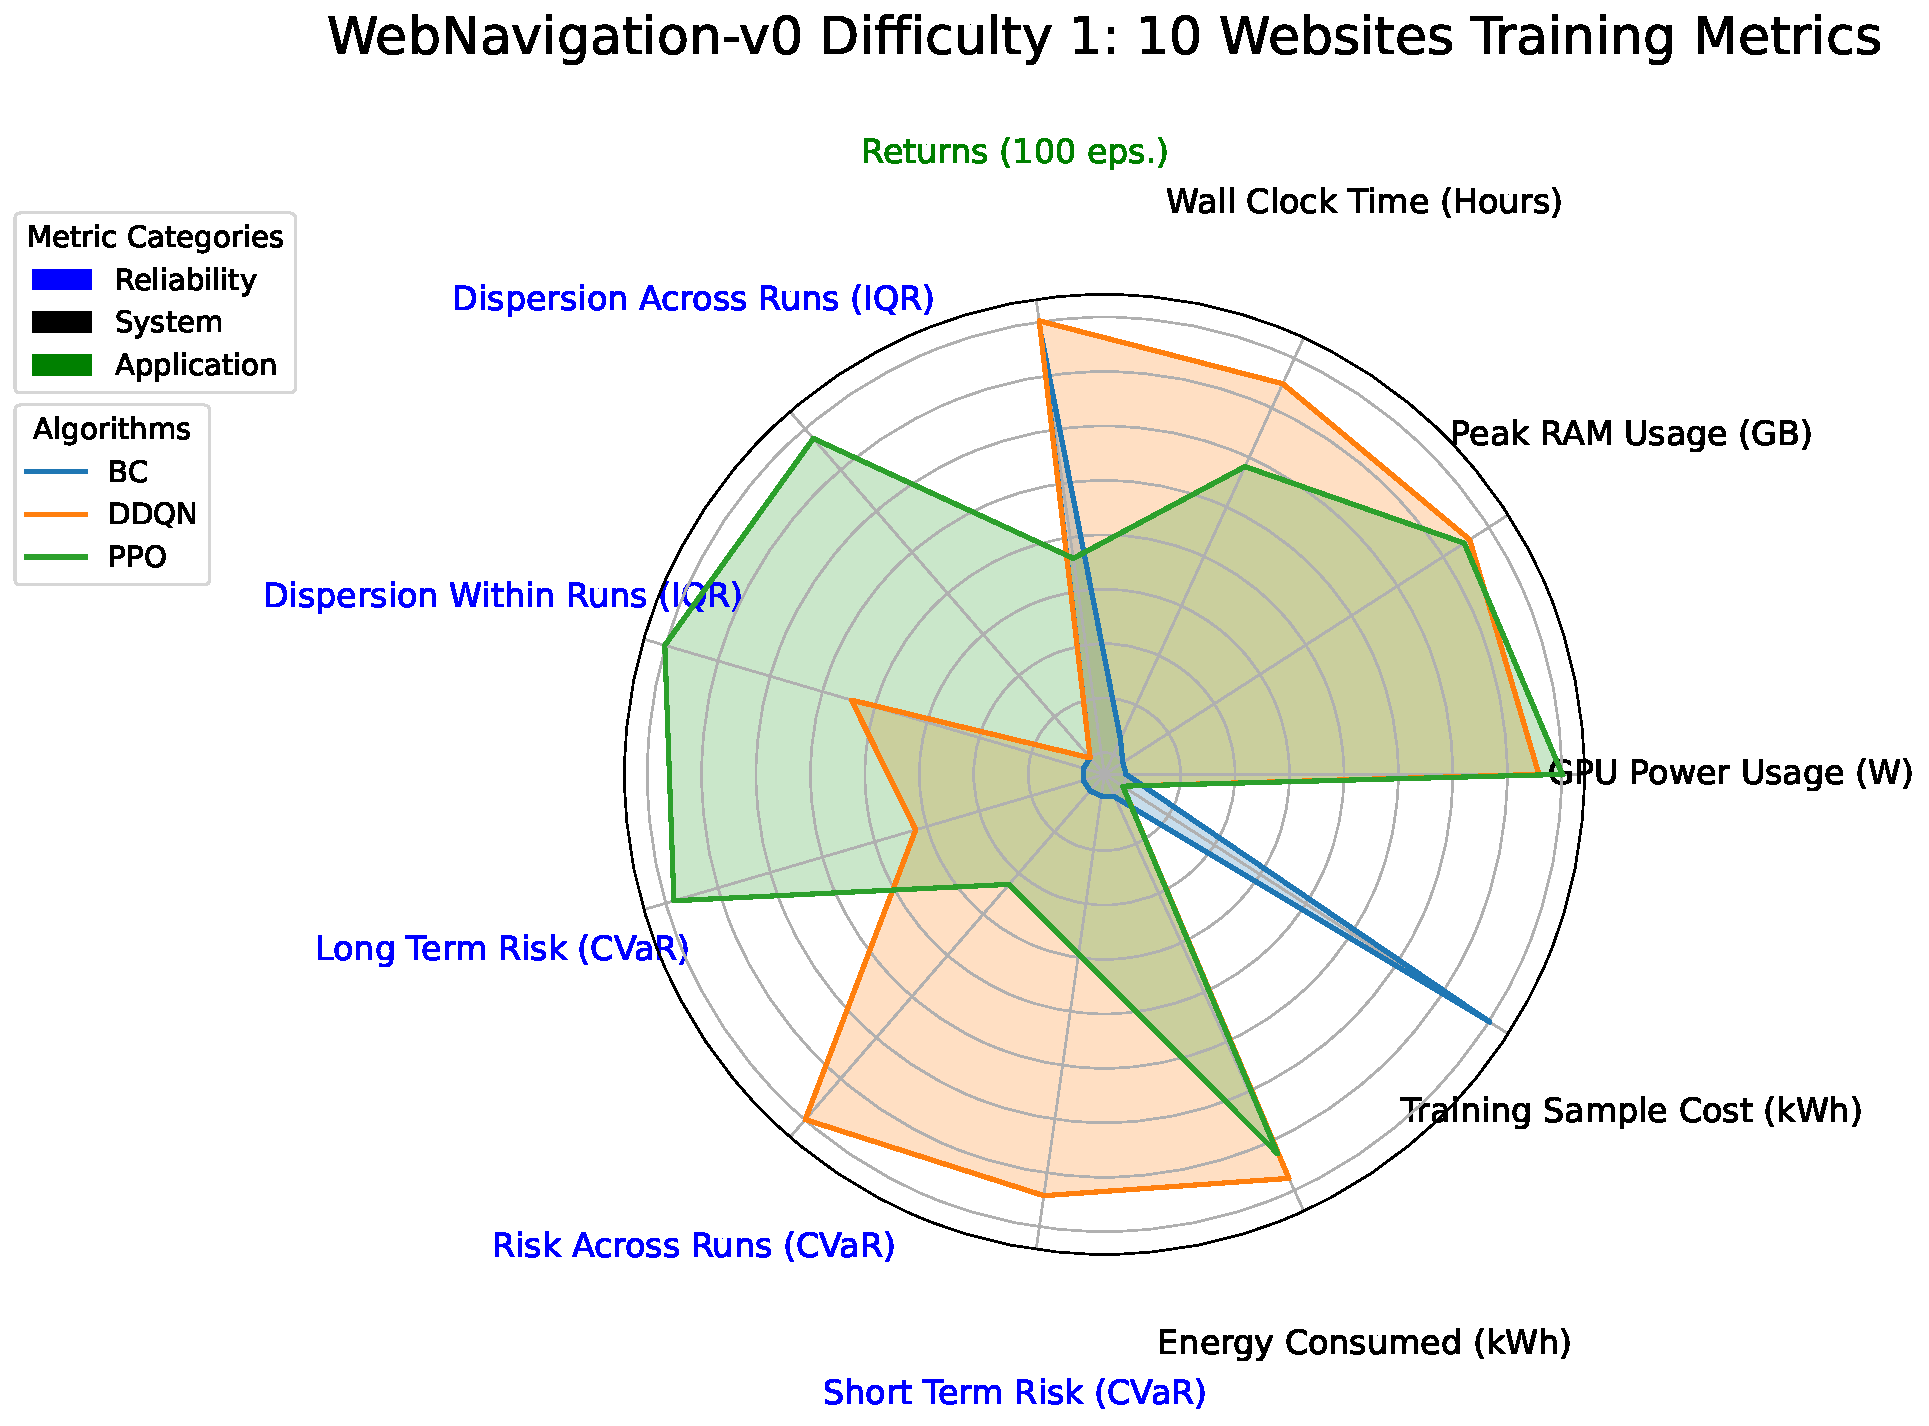
\includegraphics[width=\linewidth]{img/web_nav/WebNavigation-v0 Difficulty 1_ 10 Websites Training Metrics.pdf}
  \end{minipage}
  \hfill % optional; adds horizontal spacing
  \begin{minipage}[b]{0.4625\linewidth}
    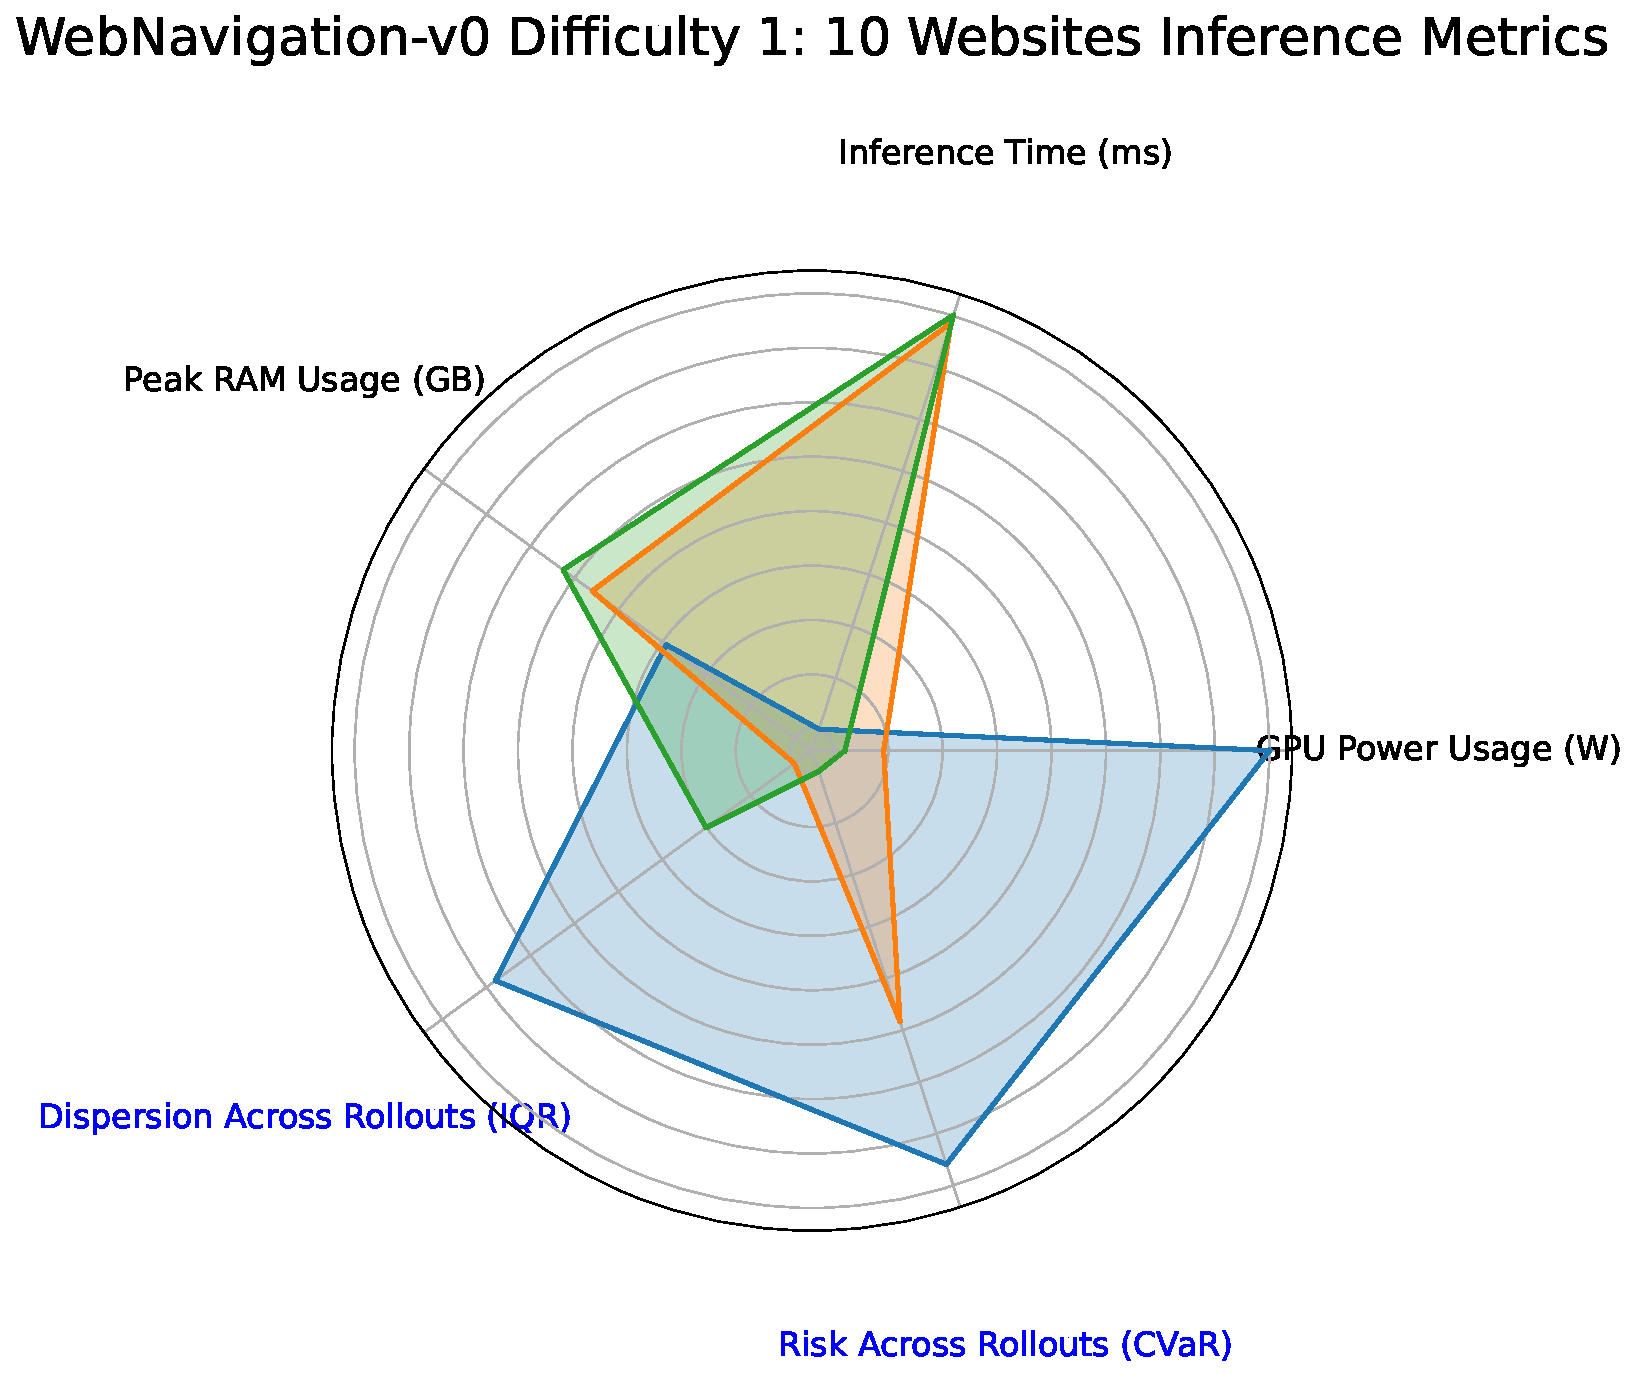
\includegraphics[width=\linewidth]{img/web_nav/WebNavigation-v0 Difficulty 1_ 10 Websites Inference Metrics.pdf}
  \end{minipage}
  \caption{Graphical representation of metrics for the "difficulty 1, 10 websites" task of WebNavigation-v0}
  \label{fig:appendix_radar_web_nav_difficulty1_10websites}
\end{figure}

